%\immediate\write18{makeindex finalthesis.nlo -s nomencl.ist -o finalthesis.nls}
\documentclass[12pt,a4paper]{report}
\usepackage[utf8]{inputenc}
%\usepackage{vietnam}
\usepackage[english]{babel}
\usepackage[left=3cm, right=2.2cm, top=2.5cm, bottom=2.5cm]{geometry}
\usepackage{amsmath}
\usepackage{float}
\usepackage{amssymb} 
\usepackage{amsfonts} 
\usepackage{graphicx} 
\usepackage[hidelinks, unicode]{hyperref}
\usepackage[labelsep=period]{caption}
\usepackage[table]{xcolor}
\usepackage{titletoc}
\usepackage{etoc}
\usepackage{mathptmx}
\usepackage{sectsty}
\usepackage{multirow}
\usepackage{booktabs, tabularx}
\usepackage{courier}
%\usepackage{subfig}
\usepackage{nomencl}
\usepackage{titlesec}
\usepackage{enumitem}
\usepackage{anyfontsize}
\usepackage[fontsize=13pt]{scrextend}
\newcommand{\code}[1]{\texttt{#1}}
\renewcommand{\baselinestretch}{1.5}
\renewcommand{\nomname}{Abbreviations} %set name of nomenclature
\usepackage{nomencl}
%\renewcommand{\thechapter}{Chapter}
\usepackage{subfigure}
\usepackage[toc,page]{appendix}
\usepackage{adjustbox}

\usepackage{longtable}
\usepackage{tikz}

\usepackage[font=small,skip=1pt]{caption}



\pagestyle{empty}
\def\layersep{2.5cm}

\makenomenclature
\makeindex

\makeatletter
\titlecontents{chapter}[3cm] % <-- seems to set some specific left margin
{\color{black}\bfseries\addvspace{3mm}}
{\makebox[0cm][r]{\MakeUppercase\@chapapp\hspace{.5em}\thecontentslabel\hspace{0.75cm}}}
{} %     ^^^ pretendously zero width box puts its contents in the left margin
{\hfill\makebox[-2cm]{\thecontentspage}}  % 3cm = twice 1.5cm
\chapternumberfont{\Large}
\chaptertitlefont{\Large}

\titleformat{\chapter}[hang] 
{\normalfont\fontsize{10}{15}\bfseries}{\thechapter.}{1em}{} 
\titlespacing*{\chapter}{0pt}{-7pt}{7pt}

\titleformat{\chapter}[hang]{\normalfont\Large\bfseries\raggedright}{\chaptertitlename\ \thechapter.}{1em}{}


\titleformat{\section}
{\normalfont\fontsize{13}{15}\bfseries}{\thesection.}{1em}{}
\titlespacing*{\section}{0pt}{-5pt}{-6pt}  

\titleformat{\subsection}
{\normalfont\fontsize{13}{15}\bfseries\itshape}{\thesubsection.}{1em}{}
\titlespacing*{\subsection}{0pt}{-5pt}{-6pt}

\titleformat{\subsubsection}
{\normalfont\fontsize{13}{15}\itshape}{\thesubsubsection.}{1em}{}
\titlespacing*{\subsubsection}{0pt}{-5pt}{-6pt}


\newcommand{\subsubsubsection}[1]{\paragraph{#1}\mbox{}\\}
%\titlespacing*{\subsection}
  %{0pt}{2\baselineskip}{3\baselineskip}

\setlist[itemize]{itemsep=-0.3em, topsep=0pt}
\setlength\parindent{0pt}
\setlength{\parskip}{10pt}
\setcounter{secnumdepth}{4}
\setcounter{tocdepth}{4}
\geometry{letterpaper}

% \title{\textbf{ĐỒ ÁN CÔNG NGHỆ MỎ}}
% \author{Bùi Trọng Nghĩa\\Diệp Công Trứ}
%\pagestyle{empty}
\pagestyle{plain}
\begin{document}
\pagenumbering{gobble}

%\pagenumbering{roman}
%\clearpage

\pdfbookmark{\contentsname}{content}
% \maketitle

\begin{center}
	\centering
	\text{THE THESIS IS COMPLETED AT}\\ 
	\textbf{PETROVIETNAM UNIVERSITY}
\end{center}
Supervisor: ..................................................\\
%(\textit{Ghi rõ họ, tên, học hàm, học vị})\\
\newline
Co-supervisor:......................................\\
%(\textit{Ghi rõ họ, tên, học hàm, học vị})\\
\newline
Thesis examiner:....................................................\\
%(\textit{Ghi rõ họ, tên, học hàm, học vị})\\
\newline
\newline
\newline
\newline
\newline
\newline
The thesis is defended at:
\begin{center}
	\centering
	\textbf{THESIS COUNCIL}\\
	\textbf{PETROVIETNAM UNIVERSITY}\\
	Month .... Date .... Year ....
\end{center}


\newpage
\begingroup
\fontsize{10pt}{12pt}\selectfont
PETROVIETNAM OIL AND GAS GROUP \hspace*{1.5cm} \textbf{SOCIALIST REPUBLIC OF VIETNAM}\\
\hspace*{.5cm}\underline{\textbf{PETROVIETNAM UNIVERSITY}} \hspace*{2.4cm} \underline{\textbf{Independence - Freedom - Happiness}}
\endgroup

\begin{center}
	\centering
	\textbf{THESIS ASSIGNMENT FORM}
\end{center}

\textbf{Student name:} Luong Khanh Loc \hspace*{2.4cm}\textbf{Student ID:} 04PET110009\\
\textbf{Major:} Petroleum engineering. \hspace*{3cm}\textbf{Class:} K4KKT\\
\textbf{1. Thesis title:}  Applied machine learning and deep learning to predict production rate.\\
\textbf{2. Assignment:} \\
\hspace*{1cm}- Study on the theory of production forecasting from conventional decline curve analysis, type curve analysis to reservoir modeling. \\
\hspace*{1cm}- Study on the data cleaning and analysis of production well.\\
\hspace*{1cm}- Building machine learning and deep learning models in predicting production rate.\\
\hspace*{1cm}- Implementation of both conventional and modern methods in excel and python.\\
\hspace*{1cm}- Optimizing several hyperparameters on machine learning and deep learning models in finding the best combination for prediction.\\
\textbf{3. Starting date: }20/03/2019\\
\textbf{4. Finishing date: }17/07/2019\\
\textbf{5. Supervisor’s name: }
	\begin{itemize}
		\item Dr. Nguyen Van Hung
		\item MSc. Luong Hai Linh
	\end{itemize}
\begin{flushright}
Ba Ria - Vung Tau, \today
\end{flushright}
\begingroup
\fontsize{12pt}{12pt}\selectfont
\textbf{RECTOR} \hspace*{70pt} \textbf{HEAD OF OFFICE OF} \hspace*{70pt} \textbf{DEAN OF PETROLEUM }\\
\hspace*{128pt} \textbf{ACADEMIC AFFAIRS} \hspace*{100pt} \textbf{FACULTY}
%(Ký, ghi rõ họ tên) \hspace{60pt} (Ký, ghi rõ họ tên) \hspace{80pt} (Ký, ghi rõ họ tên)
\endgroup

\newpage
\begingroup
\fontsize{10pt}{12pt}\selectfont
PETROVIETNAM OIL AND GAS GROUP \hspace*{1.5cm} \textbf{SOCIALIST REPUBLIC OF VIETNAM}\\
\hspace*{0.5cm}\underline{\textbf{PETROVIETNAM UNIVERSITY}} \hspace*{2.4cm} \underline{\textbf{Independence - Freedom - Happiness}}
\endgroup

\begin{center}
	\centering
	\textbf{THESIS EVALUATION FORM}\\
	%\textbf{(Giáo viên ghi nhận xét của mình, bằng tay, vào phần này)}
\end{center}

\textbf{Thesis title:} Applied machine learning and deep learning to predict production rate.\\
\textbf{Student name:} Luong Khanh Loc.\\
\textbf{Major:} Petroleum engineering \hspace*{3cm}\textbf{Course:} 2014 - 2019.\\
\textbf{Thesis examiner's name:}
\newline
\begin{enumerate}
	\item[1.] Comment on the student’s attitude of work and study:\\
	........................................................................................................................................\\........................................................................................................................................\\........................................................................................................................................\\........................................................................................................................................\\........................................................................................................................................
	\item[2.] Comment on the result:\\
	........................................................................................................................................\\........................................................................................................................................\\........................................................................................................................................\\........................................................................................................................................\\........................................................................................................................................
	\item[3.] Defects (If any):\\
	........................................................................................................................................\\........................................................................................................................................\\........................................................................................................................................\\........................................................................................................................................\\........................................................................................................................................
	\item[4.] Grade:\\
	
\end{enumerate}
\begin{flushright}
Ba Ria - Vung Tau, \today
\end{flushright}
\hspace{300pt} \textbf{SUPERVISOR}\\
%\hspace*{316pt} (Ký, ghi rõ họ tên)
\newpage
%\pagenumbering{roman}



\newpage
\begingroup
\fontsize{10pt}{12pt}\selectfont
PETROVIETNAM OIL AND GAS GROUP \hspace*{1.5cm} \textbf{SOCIALIST REPUBLIC OF VIETNAM}\\
\hspace*{0.5cm}\underline{\textbf{PETROVIETNAM UNIVERSITY}} \hspace*{2.4cm} \underline{\textbf{Independence - Freedom - Happiness}}
\endgroup

\begin{center}
	\centering
	\textbf{THESIS EVALUATION FORM}\\
	%\textbf{(Giáo viên ghi nhận xét của mình, bằng tay, vào phần này)}
\end{center}

\textbf{Thesis title:} Applied machine learning and deep learning to predict production rate.\\
\textbf{Student name:} Luong Khanh Loc.\\
\textbf{Major:} Petroleum engineering \hspace*{3cm}\textbf{Course:} 2014 - 2019.\\
\textbf{Thesis examiner's name:}
\newline
\newline
\textbf{I. COMMENT SECTION}
\begin{enumerate}
	\item[1.] Form and structure of the thesis:\\
	........................................................................................................................................\\........................................................................................................................................\\........................................................................................................................................\\........................................................................................................................................\\........................................................................................................................................
	\item[2.] Contents: 
	\begin{enumerate}
		\item[2.1] Comment on references:
	\end{enumerate}
	\item[] ........................................................................................................................................\\........................................................................................................................................\\........................................................................................................................................\\........................................................................................................................................\\........................................................................................................................................
	\begin{enumerate}
		\item[2.2] Comment on the research method:
	\end{enumerate}
	\item[] ........................................................................................................................................\\........................................................................................................................................\\........................................................................................................................................\\........................................................................................................................................\\........................................................................................................................................
	\begin{enumerate}
		\item[2.3] Comment on the result:
	\end{enumerate}
	\item[] ........................................................................................................................................\\........................................................................................................................................\\........................................................................................................................................\\........................................................................................................................................\\........................................................................................................................................
	\begin{enumerate}
		\item[2.4] Comment on the conclusion:
	\end{enumerate}
	\item[] ........................................................................................................................................\\........................................................................................................................................\\........................................................................................................................................\\........................................................................................................................................\\........................................................................................................................................
	\begin{enumerate}
		\item[2.5] Defects of the thesis:
	\end{enumerate}
	\item[] ........................................................................................................................................\\........................................................................................................................................\\........................................................................................................................................\\........................................................................................................................................\\........................................................................................................................................
\end{enumerate}
\textbf{II. GRADE:}....................................................\textit{(In words)}
\begin{flushright}
Ba Ria - Vung Tau, \today
\end{flushright}
\hspace{300pt} \textbf{THESIS EXAMINE}\\
%\hspace*{316pt} (Ký, ghi rõ họ tên)


%---------------------------------------------------------------------------------------------


%\clearpage
%\pagenumbering{roman}
%\pagestyle{empty}

%\setcounter{page}{3}
\newpage

\begin{center}
	\centering
	\textbf{STATUTORY DECLARATION}
	\addcontentsline{toc}{section}{\textbf{STATUTORY DECLARATION}}
\end{center}
I herewith formally declare that I myself wrote the submitted thesis independently and used plenty of sources mentioned at the end of this paper. I did not violate the intellectual property law and Vietnam law. I take full responsibility before the law of them..\\
\newline
\hspace*{295pt} \textbf{AUTHOR}\\
%\hspace*{280pt} (Ký, ghi rõ họ tên)
\newline
\newline
\hspace*{282pt} \textit{Luong Khanh Loc}
\pagenumbering{roman}

\newpage
\begin{center}
	\centering
	\textbf{ABSTRACT}
	\addcontentsline{toc}{section}{\textbf{ABSTRACT}}
\end{center}

\begin{center}
	\centering
	\textbf{APPLIED MACHINE LEARNING AND DEEP LEARNING TO PREDICT PRODUCTION RATE}
\end{center}
\textbf{Student name:} Luong Khanh Loc \hspace*{2.4cm}\textbf{Course:} 2014 - 2019\\
\textbf{Major:} Petroleum engineering. \hspace*{3cm}\textbf{Supervisor:} Dr. Nguyen Van Hung\\
\textbf{Class:}  K4KKT \hspace*{5.8cm} \textbf{Co-supervisor:} MSc. Luong Hai Linh\\

Recently, artificial intelligent (AI) has gained a great deal of attention in many areas, especially the oil and gas industry. There was a significant development of AI that enables oil and gas companies to reduce a huge amount of cost and make more accurate decisions. In this paper, a new method based on Artificial Intelligence including machine learning and deep learning techniques has applied to petroleum engineering to predict oil and gas production.\\
Production rates are predicted using various algorithms based on AI technique. This study proposed a novel approach using regression algorithms and ensemble methods to leverage the results. A novel method of using recurrent neural networks include long short term memory (LSTM), gated recurrent unit (GRU) and simple recurrent neural networks (Simple RNN) has been developed to predict oil and gas production. \\
Long short term memory has been chosen to compare with conventional decline curve analysis and reservoir modeling method. The outcome showed that the development of long short term memory has outperformed DCA and give better result than eclipse model in some cases.
This research focuses on figuring out the potential and efficiency of machine learning and deep learning algorithms to predict production in the future. This study explored twelve different machine/deep learning algorithms and their performance evaluation. Python is chosen for the implementation because of its useful and robust machine/deep learning libraries.


\newpage

\begin{center}
	\centering
	\textbf{ACKNOWLEDGMENTS}
	\addcontentsline{toc}{section}{\textbf{ACKNOWLEDGMENTS}}
\end{center}

First of all, I would like to express my gratitude and appreciate to all the professors and teachers and of Drilling and Production Department of PetroVietnam University who have supported me during my five-year learning at PetroVietnam university. I also thank Vietsovpetro Joint Venture, particularly Production Operations Department for giving me a precious internship which brought me a lot of experience and orientation for my graduate thesis.\\
My thanks especially go to Dr. Hung Nguyen Van who has given me immense and thoughtful knowledge and also detailed guidance. His kindly support and thorough advice went through the process of conducting my thesis had significantly enriched and improved my work. My co-supervisor, MSc. Luong Hai Linh has been extremely supportive and available whenever needed. She is always open to talk, very understanding and willing to help. I also want to thank MSc. Nguyen Viet Khoi Nguyen for the help with eclipse simulator and clear explanation of Eclipse files.\\
Additionally, I would like to express my sincere thanks to all the teachers and my friends at PVU who have giving their support during my study here. With them, my university life would be easier and meaningful. Finally, I am honored to have been a student at PetroVietnam University.\\
Once again, I would like to acknowledge and thank all of them who have helped me complete my graduate thesis.\\
Lastly, I want to dedicate this work for my families who have fully supported me during my university time.
\begin{flushright}
Luong Khanh Loc
\end{flushright}


\newpage
%\addcontentsline{toc}{chapter}{ABSTRACT}

\tableofcontents
\addcontentsline{toc}{section}{\textbf{TABLE OF CONTENTS}}

%\addcontentsline{toc}{section}{\textbf{STATUTORYDECLARATION}}
%\addcontentsline{toc}{section}{\textbf{ABSTRACT}}
%\addcontentsline{toc}{section}{\textbf{ACKNOWLEDGMENTS}}

\listoftables
\addcontentsline{toc}{section}{\textbf{LIST OF TABLES}}

\listoffigures
\addcontentsline{toc}{section}{\textbf{LIST OF FIGURES}}

%table of abbreviation
\nomenclature{$D$}{Decline rate}%
\nomenclature{$b$}{ Arps’ decline curve exponent}%
\nomenclature{$a$}{The number of angels per unit area}%
\nomenclature{$N$}{The number of angels per needle point}%
\nomenclature{$A$}{The area of the needle point}%
\printnomenclature
\addcontentsline{toc}{section}{\textbf{ABBREVIATIONS}}
\nomenclature{$\mathbf{X}$}{The input data for machine learning algorithms}
\nomenclature{$\mathbf{w}$}{The learning parameters for machine learning algorithms}
\nomenclature{$y$}{Actual value of production rate}
\nomenclature{AI}{Artificial Intelligent}%
\nomenclature{DCA}{Decline Curve Analysis}%
\nomenclature{SEPD}{Stretched Exponential Production Decline}%
\nomenclature{LSTM}{Long Short Term Memory}%
\nomenclature{GRU}{Gated Recurrent Unit}%
\nomenclature{RNN}{Recurrent Neural Networks}%
\nomenclature{XGB}{Extreme Gradient Boosting}%
\nomenclature{LGBM}{Light Gradient Boosting Machine}%
\nomenclature{MLP}{Multi Layers Perceptron}%
\nomenclature{BHP}{Bottom Hole Pressure}%
\nomenclature{THP}{Tubing Head Pressure}%
\nomenclature{BHT}{Bottom Hole Temperature}%
\nomenclature{WHT}{Well Head Temperature}%
\nomenclature{DP}{Different Pressure in casing}%
\nomenclature{CS}{Choke Size (Percentage)}%
%\printnomenclature

\newpage
\begin{center}
\textbf{PREFACE}
\end{center}
\addcontentsline{toc}{section}{\textbf{PREFACE}}
\textbf{Rationale}\\
Production forecasting is one of the most difficult tasks in petroleum engineering. Its purpose has been significantly important for making decision related to business development. There various way to predict future production includes traditional decline curve analysis (DCA), type curve and reservoir modeling. Recently, with the development of artificial intelligence, AI can improve their capacity in prediction. So, the potential and efficiency of AI technique have been studied in this work.\\
\textbf{Objective}
\begin{itemize}
	\item Study on the theory of production forecasting from conventional decline curve analysis, type curve analysis to reservoir modeling.
	\item Study on the data cleaning and analysis of production well.
	\item Building machine learning and deep learning models in predicting production rate.
	\item Implementation of both conventional and modern methods in excel and python.
	\item Optimizing several hyperparameters on machine learning and deep learning models in finding the best combination for prediction.
\end{itemize}
\textbf{Subject and scope}
\begin{itemize}
	\item Subject: Production prediction with decline curve analysis, reservoir modeling and artificial intelligence methods. 
	\item Scope: This thesis is work on Volve filed which is a decommissioned field located in North Sea, specifically five production wells are used to predict the future production rate.
\end{itemize}
\textbf{Methodology}
\begin{itemize}
	\item Reading documents related to the oil and gas production forecasting, reservoir modeling and artificial intelligence methods applied in petroleum engineering.
	\item Building a work-flow for using machine learning and deep learning algorithms in production prediction and implementation in python library.
	\item Making comparison between three methods (conventional DCA, reservoir modeling and artificial intelligence) in order proving the potential of AI that can be an effective tools in oil and gas industry.
\end{itemize}
\textbf{Significance}
\begin{itemize}
	\item Scientific significance: The thesis presents theories about production analysis, machine learning, and deep learning algorithms, especially reveal the great performance of artificial intelligence methods in term of production forecasting. Also, the thesis could possibly be a reference source for those who want to explore the potential of AI when applying to petroleum engineering.
	\item Practical significance: This is a piece of work that proves the novel methods of using artificial intelligence including machine and deep learning can be tools for engineering in production prediction.
\end{itemize}
\textbf{Thesis structure}\\
\textbf{Chaper 1: Overview of production forecasting}
\begin{itemize}
	\item History of production analysis
	\item Traditional decline curve methods
	\item Type curve methods
	\item Reservoir modeling and forecast methods
\end{itemize}
\textbf{Chapter 2: Overview of Volve field}
\begin{itemize}
	\item Field description
	\item Reservoir
	\item Production profile
\end{itemize}
\textbf{Chapter 3: Artificial Intelligence}
\begin{itemize}
	\item Machine learning
	\item Deep learning
\end{itemize}
\textbf{Chapter 4: Methodology}
\begin{itemize}
	\item Input data
	\item Work-flow
\end{itemize}
\textbf{Chapter 5: Result and discussion}
\begin{itemize}
	\item Machine learning output
	\item Deep learning output
	\item Applied LSTM
\end{itemize}
\textbf{Chapter 6: Conclusion}\\
\textbf{Appendix A. Preprocessing and data used in thesis}\\
\textbf{Appendix B. Hyperparameters optimization}\\
\textbf{Appendix C. Machine learning result}\\
\textbf{Appendix D. Results of LSTM on five well}\\
\textbf{Appendix E. Results of LSTM cumulative gas and water}
	



\pagenumbering{arabic}
%\newpage

\chapter{Overview of production forecasting}
\section{History of production analysis\cite{Hedong}}
The Production Analysis started in 1920 with a pure motive to find the best decline function by which it is possible to predict the revenue of the production in the future on an empirical basis with no technical background in it. Then (Arps , 1945) formulated the constant pressure exponential, hyperbolic and harmonic rate decline. In 1960, Type-curves were first introduced, still assuming constant flowing pressure by Fetkovich. These type-curves have two families one related the transient flowing period and the other for the late boundary- dominated flow. In late 80s and early 90s, (Palacio \& Blasingame, 1993) introduces the variable rate/variable pressure type-curves as a log-log plot of productivity index vs material balance time.\\
Currently, the production decline analysis technique consists of the conventional Arps (1945) method, classical Fetkovich (1980) type curve matching method, modern Palacio and Blasingame (1993) and Agarwal et al. (1998) type curve matching methods and FMB (1998) reservoir engineering method.\\
Extrapolating the characteristic trend of some variables of a well can be helpful for our jobs. As to a well, the simplest and the most easily available variable is its production. If the flow rate versus time or cumulative production curve is plotted and extrapolated, the ultimate cumulative production can be obtained. The trend or mathematical relations indicated by the entire rate history of a well can be used to fore- cast the production performance in the future, which is referred to as the conventional Arps (1945) decline curve analysis method. This method magnificently describes the production decline laws of well at a constant bottom hole flowing pressure (BHFP) and in the completely boundary-dominated flow period. The greatest advantage of this method is that formation parameters are not necessarily obtained. On the other hand, it is not suitable for data analysis from the transient flow stage.\\
Arps type curve can only be used to analyze the data of a boundary-dominated flow period. Fetkovich (1980), on the basis of homogeneous bounded formation transient filtration theory, introduced the transient flow formula in well test analysis to the decline analysis, so that the Arps type curve is extended to the transient flow period prior to boundary-dominated flow, and the transient rate decline curve and the Arps rate decline equation are organically combined. In this way, the production decline laws and the effect of boundary are intuitively shown, and a set of relatively complete log–log production decline curve matching analysis method similar to well test analysis is developed. The greatest advantage of the method is its ability to reliably determine whether the production is in a transient flow period or in a boundary-dominated flow period.\\
Both Arps and Fetkovich methods assume that the BHFP is constant to analyze the production data without considering the change of gas pressure–volume–temperature (PVT) charateristics with pressure. Palacio and Blasingame (1993) introduced the pseudo-pressure normalized production $(q\Delta p_{p})$ and the material balance pseudo- time $t_{ca}$ to develop the type curve, which considered the production at variable BHFP and the gas PVT changing with formation pressure.\\
Agarwal et al. (1998) used the relations of pseudo-pressure normalized production $(q\Delta p_{p})$ , material balance pseudo-time $t_{ca}$, and dimensionless parameters in well test analysis to develop the Agarwal-Gardner production decline analysis. Owing to the different definitions of dimensionless quantity, the early part of the curve is more discrete than the Blasingame chart and thus is in favor of reducing the ambiguity of matching analysis.\\
Both Blasingame and Agarwal-Gardner methods used the pseudo-pressure normalized production $(q\Delta p_{p})$ and the material balance pseudo-time $t_{ca}$ to create type curve, while the NPI (normalized pressure integral) method (Blasingame et al., 1989) used the production normalized pressure integral to analyze the data available, which was not affected by the scatter of data.\\
Palacio and Blasingame (1993) and Agarwal et al. (1998) type curve matching analysis methods introduced pseudo-time (or material balance pseudo-time) and production normalized pseudo-pressure (pseudo-pressure normalized production) to deal with variable BHFP, variable rate, and change of gas PVT with pressure. They used the flow rate integral, flow rate integral derivative, cumulative production–time, and flow rate–cumulative production type curves as the auxiliary matching analysis curves to reduce the ambiguity of interpretation results.\\
Mattar et al. (1998, 2006) and Agarwal et al. (1998) suggested using the “flow (dynamic) material balance” method to analyze the production data, and conduct- ed detailed discussion on the calculation of material balance time. This method is simple and easy. Mattar and Anderson (2003) believes that there is no one universal production data analysis method that can meet all types of reservoirs, and the best way to eliminate analysis errors is to synthetically use all analysis methods and consider flowing pressure data.\\
Over nearly a century, the Production Analysis technique has evolved with several advances, including target to be analyzed, that is, from purely production data to both flow rate and pressure data; analytic model, that is, from no model to both analytical model and numerical model; analytic method, that is, from the empirical Arps method to the log-log method represented by Blasingame; applicable conditions, that is, from simple constant pressure production data to variable pressure and variable rate data; and the estimation parameters, that is, from only cumulative production to many parameters such as formation permeability, skin factor, dynamic reserves and drainage area, as well as interwell communication and infill potential.
\section{Traditional decline curve methods\cite{Tarek}}
Decline curves are one of the most extensively used forms of data analysis employed in evaluating gas reserves and predicting future production. The decline-curve analysis technique is based on the assumption that past production trends and their controlling factors will continue in the future and, therefore, can be extrapolated and described by a mathematical expression.\\
The method of extrapolating a “trend” for the purpose of estimating future performance must satisfy the condition that the factors that caused changes in past performance, for example, decline in the flow rate, will operate in the same way in the future. These decline curves are characterized by three factors:
\begin{itemize}
	\item Initial production rate, or the rate at some particular time
	\item Curvature of the decline
	\item Rate of decline
\end{itemize}
Arps (1945) proposed that the “curvature” in the production-rate versus time curve can be expressed mathematically by a member of the hyperbolic family of equations. Arps recognized the following three types of rate-decline behavior:
\begin{itemize}
	\item Exponential decline
	\item Harmonic decline
	\item Hyperbolic decline
\end{itemize}
Each type of decline curve has a different curvature, as shown in Figure 1-1. This figure depicts the characteristic shape of each type of decline when the flow rate is plotted versus time or versus cumulative production on Cartesian, semi log, and log-log scales. The main characteristics of these decline curves can be used to select the flow rate decline model that is appropriate for describing the rate–time relationship of the hydrocarbon system:
\begin{figure}[H]
\centering
\includegraphics[scale = 0.6]{Fig_theo/decline}
\caption{Classification of production decline curves}
\end{figure}
\begin{enumerate}
	\item \textbf{Exponential decline:}
	 A straight-line relationship will result when the flow rate versus time is plotted on a semi log scale and also when the flow rate versus cumulative production is plotted on a Cartesian scale.
	\item \textbf{Harmonic decline:}
	Rate versus cumulative production is a straight
	line on a semi log scale; all other types of decline curves have some curvature. There are several shifting techniques that are designed to straighten out the curve that results from plotting flow rate versus time on a log-log scale.
	\item \textbf{Hyperbolic decline:}
	None of the above plotting scales, that is, Cartesian, semi log, or log-log, will produce a straight-line relationship for a hyperbolic decline. However, if the flow rate is plotted versus time on log-log paper, the resulting curve can be straightened out with shifting techniques.
\end{enumerate}
The decline-curve analysis is based on empirical relationships of production rate versus time, given by Arps (1945) as follows:
\begin{equation}
q_{t} = \frac{q_{i}}{(1+bD_{i}t)^{\frac{1}{b}}}
\end{equation}
where:
\begin{enumerate}
	\item[] $q_{t}$ is flow rate at time t, m3/day
	\item[] $q_{i}$ is initial flow rate, m3/day
	\item[] t is time, day
	\item[] $D_{i}$ is initial decline rate, $day^{-1}$
	\item[] b is Arps' decline curve exponent
\end{enumerate}
The decline rate D is defined as the rate of change of the natural loga- rithm of the production rate, that is, ln(q), with respect to time, t
\begin{equation}
D = -\frac{d(lnq)}{dt} = -\frac{1}{q}\frac{dq}{dt}
\end{equation}
The minus sign has been added because dq and dt have opposite signs and it is convenient to have D always positive. Notice that the decline- rate equation, Equation 1-2, describes the instantaneous changes in the slope of the curvature, dq/dt, with the change in the flow rate, q, over time.\\
The parameters determined from the classical fit of the historical data, namely the decline rate, D, and the exponent, b, can be used to predict future production. This type of decline-curve analysis can be applied to individual wells or the entire reservoir. The accuracy of the entire reservoir application is sometimes even better than for individual wells due to smoothing of the rate data. Based on the type of rate-decline behavior of the hydrocarbon system, the value of b ranges from 0 to 1, and, accordingly, Arps’s equation can be conveniently expressed in the following three forms:
% Please add the following required packages to your document preamble:
% \usepackage{booktabs}
\begin{table}[H]
\centering
\caption{Different values b versus three kinds of decline curve}
\begin{tabular}{@{}lll@{}}
\toprule
\textbf{Case}        & \textbf{b}                & \textbf{Rate-time relationship}                   \\ \midrule
\textbf{Exponential} & b = 0                     & $q_{t} = q_{i}exp(-D_{i}t)$                       \\
\textbf{Hyperbolic}  & 0\textless{}b\textless{}1 & $q_{t} = \frac{q_{i}}{(1+bD_{i}t)^{\frac{1}{b}}}$ \\
\textbf{Harmonic}    & b = 1                     & $q_{t} = \frac{q_{i}}{(1+bD_{i}t)}$               \\ \bottomrule
\end{tabular}
\end{table}

A recomendation for b value is given by the table below:
% Please add the following required packages to your document preamble:
% \usepackage{multirow}
% Please add the following required packages to your document preamble:
% \usepackage{booktabs}
% \usepackage{multirow}
\begin{table}[H]
\centering
\caption{Recomedation of b values}
\begin{tabular}{@{}ll@{}}
\toprule
\textbf{b values}               & \textbf{System Characterization and Identification}                          \\ \midrule
\multirow{7}{*}{0}              & Gas wells undergoing liquid loading                                          \\
                                & Wells with high back pressure                                                \\
                                & High-pressure gas                                                            \\
                                & Low-pressure gas with a back-pressure curve exponent of n $\sim$0.5          \\
                                & Poor waterflood performance (oil wells)                                      \\
                                & Gravity drainage with no solution gas (oil wells)                            \\
                                & Solution gas drive with unfavorable kg/ko (oil wells)                        \\
0.3                             & Typical for solution-gas-drive reservoirs                                    \\
0.4 - 0.5                       & Typical for gas wells, b = 0.5 for pwf$\sim$0;  b = 0.4 for pwf  $\sim$0.1pi \\
0.5                             & Gravity drainage WITH solution gas and for water-drive oil reservoirs         \\
\multirow{2}{*}{Undeterminable} & Constant-rate or increasing-rate production period                           \\
                                & Flow rates are all in transient or infinite-acting period                    \\
0.5 \textless b \textless 0.9   & Layered or composite reservoir                                               \\ \bottomrule
\end{tabular}
\end{table}

It should be pointed out that these three forms of decline-curve equations are applicable only when the well/reservoir is under pseudosteady (semi steady)-state flow conditions, that is, boundary-dominated flow conditions. The following is a list of inherent assumptions that must be satisfied before performance of rate–time decline-curve analysis:
\begin{itemize}
	\item The well is draining a constant drainage area, that is, the well is in a boundary-dominated flow condition.
	\item The well is produced at or near capacity.
	\item The well is produced at a constant bottom-hole pressure.
\end{itemize}
These three conditions must be satisfied before any of the decline-curve analysis methods is applied to describe the production performance of a reservoir. However, it can be extremely difficult to determine when a well has defined its drainage area and thus identification of the peseudo steady state flow condition. It is the main obstacle of using Arps's decline curve. 

\section{Type curve methods.\cite{Tarek}}
The type-curve analysis approach was introduced to the petroleum industry by Agarwal et al. (1970) as a valuable tool when used in conjunction with conventional semi log plots. A type curve is a graphical representation of the theoretical solutions to flow equations. Type-curve analysis consists of finding the theoretical type curve that “matches” the actual response from a test well and the reservoir when subjected to changes in production rates or pressures. The match can be found graphically by physical superposition of a graph of actual test data on a similar graph of type curve(s) and searching for the type curve that provides the best match. Since type curves are plots of theoretical solutions to transient and pseudosteady-state flow equations, they are usually presented in terms of dimensionless variables, for example:
\begin{itemize}
	\item dimensionless pressure, $p_{D}$
	\item dimensionless time, $t_{D}$
	\item dimensionless radius, $r_{D}$, and
	\item imensionless wellbore storage, C.
\end{itemize}
rather than real variables (e.g., $\Delta p$, t, r, and C). The reservoir and well parameters, such as permeability and skin, can then be calculated from the dimensionless parameters defining that type curve.\\
The variable can be made “dimensionless” when multiplied by a group of constants with opposite dimensions, but the choice of this group will depend on the type of problem to be solved. For example, to create the dimensionless pressure drop, $p_{D}$, the actual pressure drop $\Delta p$ in psi is multiplied by group \textbf{A} with units of $psi^{-1}$ or $p_{\Delta} = A\Delta p$. Finding a group A that makes a variable dimensionless is derived from equations that describe reservoir fluid flow.\\
A well-known Darcy's equation is expressed by:
\begin{equation}
Q = [\frac{kh}{141.2B\mu [ln(r_{e}/r_{wa}) - 0.5]}]\Delta p
\end{equation}
where $r_{wa}$ is apparent (effective) wellbore radius, defined by: $r_{wa} = r_{w} e^{-s}$.
Group A can be then defined by rearranging Darcy's equation as:
\begin{equation}
ln(\frac{r_{e}}{r_{wa}}) - \frac{1}{2} = [\frac{kh}{141.2QB\mu}]\Delta p
\end{equation}
So, $p_{D}$ is defined by:
\begin{equation}
p_{D} = [\frac{kh}{141.2QB\mu}]\Delta p
\end{equation}
Similarly, $t_{D}$ is defined by:
\begin{equation}
t_{D} = [\frac{0.0002637k}{\phi \mu c_{t}r_{w}^{2}}]t
\end{equation}
By using Ei function for solving diffusitivity equation in reservoir:
\begin{equation}
p_{r,t} = p_{i} +[\frac{70.6QB\mu}{kh}]Ei[\frac{-948\phi \mu c_{t}r_{w}^{2}}{kt}]
\end{equation}
Rewrite the equation above:
\begin{equation}
\frac{p_{i} - p_{r,t}}{[\frac{70.6QB\mu}{kh}]}  = -\frac{1}{2}Ei[\frac{-(r/r_{w})^{2}}{4\frac{0.0002637kt}{\phi \mu c_{t}r_{w}^{2}}}]
\end{equation}
From the definition of the dimensionless variables $p_{D}, t_{D}, and r_{D}$, this relation can be expressed in terms of these dimensionless variables:
\begin{equation}
p_{D} = -\frac{1}{2}Ei(\frac{-(r_{D})^{2}}{4t_{D}})
\end{equation}
By applying this similar dimensionless variables to decline curve analysis, several investigators have employed the dimensionless-variables approach to determine reserves and to describe the recovery performance of hydrocarbon systems with time, notably the following:
\begin{enumerate}
	\item Fetkovich (1980)
	\item Carter (1985)
	\item Palacio and Blasingame (1993)
	\item Mattar and Anderson’s Flowing Material Balance (2003)
	\item Anash et al. (2000)
	\item Decline-curve analysis for fractured reservoirs
\end{enumerate}
All the methods are based on defining a set of decline-curve dimension- less variables that includes:
\begin{enumerate}
	\item Decline-curve dimensionless rate, $q_{Dd}$
	\item Decline-curve dimensionless cumulative production, $Q_{Dd}$
	\item Decline-curve dimensionless time, $t_{Dd}$
\end{enumerate}
The aforementioned methods were developed with the objective of providing the engineer with an additional convenient tool for estimating reserves and determining other reservoir properties for oil and gas wells using the available performance data. A review of these methods and their practical applications is given in the book of Reservoir Engineering Handbook by Tarek \cite{Tarek}.\\
Recently, there are a significant software that cover all of this type curve analysis such as  Fekete Rate Transient Anlysis, Topaze NL-RTA by KAPPA or IHS-RTA by IHS Markit.\\
In this thesis, author has chosen traditional decline curve analysis by Arps rather than type curve analysis for making comparison with novel methods of using Artificial intelligence.





\section{Reservoir modelling and forecast methods}
Today, reservoir modeling is an essential part of every field development and assessment because of its reliability and accuracy compare with other conventional methods. In this thesis, the author does not cover the theoretical knowledge of reservoir modeling instead, by introducing some of the core function of reservoir modeling in order to compare with machine learning and deep learning methods that will cover in the next chapter.
\subsection{Reservoir modelling \cite{His1}}
In short words, the reservoir model is a computer model based on geological model. The purpose of the reservoir model is to help facilitate numerical calculations in an effective matter. To achieve this, a huge detailed geological model must go through a reduction in parameters to reduce simulation time, usually done by dividing the geological model into grid quantitative parameters from the statics geological model in addition to dynamic parameters. This makes the reservoir model a good base for consistent analysis of the hydrocarbon presents, also giving a good basis for further economical assessment. It is also used for production optimization through well placement and tertiary recovery techniques.\\
Dynamic parameters are parameters that change during production history. These could be well rates, grid block pressure, phase permeability, PVT characteristics of fluid or liquid and gas saturation. Some of the dynamic parameters, like grid block pressure, can vary significantly during years, or even months, of production. Matching these parameters are very challenging, as one during production does not have data specific to one grid cell. but rather data only from production and injection wells which is a result of actions from many grid-block. Static parameters, like mineralogy and net to gross ratio, do not change during production history. These kinds of parameters should thus be easier to model, as they would have the same value during the entire history matching period.\\
With all these parameters that needs to be defined, data is acquired from several different sources in the petroleum industry. Each type of data has a certain spatial extent associated to it. A large-scale geophysical survey, like seismic survey, could provide us with rock-types, fault placement and in some cases porosity estimates. These data does not reveal much of the heterogeneity within a cubic meter of rocks. Through well tests one can get estimates of the product of permeability and skin or near well-bore effects of the reservoir, but as with geophysical data these data are a sum of actions across a large volume of reservoir, so does not explain the actual parameters in one region or in one grid cell. Further data collection through well logs and core samples could give data like net to gross ratio, electric resistivity, hydrocarbon content and porosity. Applying these data to a reservoir model needs to be done with consideration to both spatial variance and measurement errors. With all this data incorporated in the model, a final quality check needs to be done in order to see whether the model is geological plausible. This requires a geological interpretation, and could be performed by seeing if porosity and permeability values are consistent with rock type \cite{His2}. \\
By using commercial reservoir simulator, we can use the reservoir model to predict future production. The accuracy of the prediction is influenced by several uncertain factors. The sources of error include, among other, the reservoir model, similator and flow physics. This prediction is often used as a basic for major reservoir development decisions and some important decision are based on the expected recovery factor from simulation.
\subsection{History matching}
History matching is one of the core activities performed by petroleum engineers to decrease the uncertainty of reservoir models. By comparing real data production data gathered at the surface, with the output from a reservoir simulator, the gaps in reservoir properties of those block cells in the model is filled.\\
The goal of history matching is to find a plausible model variable $\textbf{m}$ that minimize the square norm of the data mismatch:
\begin{equation}
J(m) = \frac{1}{2} \parallel g(\textbf{m}) - \textbf{d}_{obs}\parallel _{D} ^{2}
\end{equation}
where $g(\textbf{m})$ is the output of the model (typical output from simulated model) and $\textbf{d}_{obs}$ is the vector observed data.\\
In order to perform and achieve a history match of reservoir model some sort of historical performance data must exist. These data can be production rates of different phases, pressures or any other historic data describing reservoir performance. By constraining the wells in a simulation model with a chosen type of performance data and compare the calculated model response with historical data available, the reservoir model is able to predict future actions of reservoir, production rate and recovery factor.  Because of the uncertainty of the data, in order to get a reliable model that can be further foundation of making decision, reservoir model have to be fully understanding before running any history matching.\\
For example, we may specify the model to be simulated with well constrained by oil rate. The model will calculate the corresponding rates of gas and water according to mobility and pressure, these in turn can be compared with measured rates. The history match will be validated based on how good it matches the historical reservoir performance. There is usually some sort of deviation between the behavior of the simulation model and the actual reservoir. This established the need to predetermine a criteria used to describe a successful match.\\
\subsubsection{Manual history matching \cite{His4}}
Before automatic history matching of realistic reservoir models was feasible, reservoir models were history matched manually using good engineering judgment and a work flow that had been developed through years of experience. There were a wide range of ways to match the output of model with actual data. A typical method is begins with an attempt to match pressures at the large (field) scale through adjustments of a few key parameters: aquifer pore volume factors, aquifer transmissibility, permeability multipliers, rock compressibility, and the ratio of vertical to horizontal permeability. When the pressure has been matched adequately at the field level, the properties of individual flow units or layers are adjusted, followed by the adjustment of well properties or properties of cells near wells.
Once the pressure matching is complete, other variables are adjusted in an attempt to match water arrival times and water cut behavior. Williams et al\cite{His3} suggest that modification of the relative permeability curves is frequently useful for saturation matching because its effect on the pressure match may be relatively small. In some cases, it may be necessary to locally increase or decrease vertical transmissibility to change the flow of water from the lower layers to the upper layers in the reservoir.
\subsubsection{Automatic history matching\cite{His1}}
Automatics history matching (or assisted history matching) routines uses optimization algorithms to mathematically describe the observed mismatch and update the reservoir model. Such routines can be divided in two groups, deterministic and stochastic models. The deterministic models require calculations of Jacobian or Hessian matrices in order to approach the true solution. Stochastic models focuses on minimizing a objective function without the use of gradients. This is generally more computationally demanding because of the model parameter space being searched can be very large, but can generally be applied to non-linear cases where gradient calculations are very hard. Major challenges for both methods are the huge parameter sets, the non-linearity of reservoir simulation and several local minimas in the objective function.\\
Although the objectives of history matching are relatively consistent (minimization of the square data mismatch with regularization), the methods used for the minimization and for assessing uncertainty vary widely. 
During a past decade, there were a various implementation of algorithms in automatics history matching:
\begin{enumerate}
	\item Gradient descent methods
	\item Design of Experiments
	\item Respone surface modeling
	\item Parametric methods
	\item Ensemble Kalman Filters
	\item Artificial Intelligent methods (include ANN, GA, fuzzy logic...)
	\item Hybric methods
	\item Travel time inversion
	\item Multiple solution
\end{enumerate}
Different algorithms yield with different problems of history matching. Part of the reason for the differences is clearly that some methods are easier to implement than others, but it is also clear that different history matching problems may require different optimization algorithms. One consequence of the “no free lunch theorem for search and optimization is that “a general-purpose universal optimization strategy is theoretically impossible, and the only way one strategy can outperform another is if it is specialized to the specific problem under consideration"\cite{His4}. So, based on the kind of history matching problem, number of parameters, computational limit, convergence speed and other aspect,  in some case one algorithms can be better than the others.
\subsection{Prediction}
The objective of history matching is to provide a model than can reasonably predict the future performance of the reservoir under various operational scenarios. Different opera- tional scenarios may include well stimulations, drilling of new wells, abandonment of existing wells, injection of different fluids, and modification of surface facilities. These actions are intended to increase or accelerate hydrocarbon recovery and most will require significant capital investment. Hence, a facility for economic analysis is required in the comparison of alternative operational scenarios.\\
The development planning process is an exercise in optimization, in which the objective is to maximize economic metrics such as net present value (NPV) or ultimate recovery, while honoring the external constraints, such as physical (platform) limitations, available capital, drilling rigs, or injection gas. The nature of the objective function (i.e., NPV) must be clearly defined before the optimization stage, as it provides the means to compare different scenarios.\\
\begin{figure}[H]
\centering
\includegraphics[scale = 0.5]{Fig_theo/simulation}
\caption{Processing of using reservoir modeling}
\end{figure}
Even when a reservoir model is calibrated (history-matched), there can be many parameters of reservoir or fluid interaction parameters that may not have been tested. So a question of whether a calibrated model can be verified to predict the future actions of reservoir?






\chapter{Overview of Volve field}
\section{Field description}
Volve is a decommissioned field located in the North Sea which was revealed in 1993. The Field is situated 200 kilometers west of Stavanger at the southern terminal of the Norwegian division as shown in Figure 1 and five kilometers north of the Sleipner Ost field with water depths of 80 meters in the block 15/9. Drilling started in May 2007, came into production the following year, and ended in 2016 after 8.5 years in operation, more than twice as long as originally planned. New wells were being drilled up until 2012-13, which contributed to the increased recovery rate and extended the life of the field. However remaining resources were very limited and with the decrease in oil prices over recent years, new wells were no longer profitable. All possibilities to extend the life of the field were explored, which later yielded very good results.
\begin{figure}[H]
\centering
\includegraphics[scale = 0.5]{Volve/volve}
\caption{Location of Volve field}
\end{figure}

\subsection{Reservoir}
Volve produced oil from sandstone of Middle Jurassic age in the Hugin Formation. The reservoir is at a depth of 2,700-3,100 metres. The western part of the structure is heavily faulted and communication across the faults is uncertain.
The field was produced with water injection for pressure support.
\begin{figure}[H]
\centering
\includegraphics[width=1.0\textwidth]{Volve/0.png}
\caption{Reservoir model of Volve field}
\end{figure}
\section{Production profile}
The development was based on production from the Maersk Insprirer jack-up rig, with Navion Sga used as a storage ship to hold crude oil before export. Gas was piped to Sleipner which is a platform for final processing and export. Volve reached a recovery rate 54\% and in March 2016 the license decided to shut down its production permanently. The field was originally scheduled for 3-5 years of operation. \\
Starting in February 2008, the Volve production lasted for about eight years. At peak, the field produced 56,000 barrels per day, and a total of 63 million barrels of oil were produced before the field was shut down in 2016. The field was developed when the oil price was low, and an unconventional concept was chosen to recover the resources in an easy and profitable manner. The field data will now have a new life for the purposes of study and research after the decommissioning. The Volve licensees were ExxonMobil and Bayerngas. Information about geology, geophysics, drilling, static models, dynamic simulations and other information has provided by Equinor company in 2018\cite{Volve}.
Detailed production in each year has shown in the figure below:
\begin{figure}[H]
\centering
\includegraphics[width=1.0\textwidth]{Volve/Production}
\caption{Production during the period 2008 to 2017}
\end{figure}

\clearpage
\begin{longtable}[c]{| c | c | c |c |c |c |c |c |c |c |}

 \caption{Production profile of Volve filed.\label{long}}\\
 \toprule
 %\hline
 %\multicolumn{10}{| c |}{}\\
 %\hline
 %Something & something else\\
 %\textbf{DATE} & \textbf{BHP} & \textbf{BHT} & \textbf{DP} & \textbf{CS(\%)} & \textbf{WHP} & \textbf{WHT} & \textbf{OIL} & \textbf{GAS} & \textbf{WAT} \\
 %\hline
 %\endfirsthead
 
 %\hline
 %\multicolumn{10}{|c|}{Continuation of Table \ref{long}}\\
 %\hline
 %Something & something else\\
 \textbf{DATE} & \textbf{BHP} & \textbf{BHT} & \textbf{DP} & \textbf{CS(\%)} & \textbf{WHP} & \textbf{WHT} & \textbf{OIL} & \textbf{GAS} & \textbf{WAT} \\\midrule
 %\hline
 %\endhead
 
 %\hline
 %\endfoot
 
 %\hline
 %\multicolumn{10}{| c |}{End of Table}\\
 %\hline\hline
 %\endlastfoot
 
1/30/09       & 257.44       & 105.34       & 163.29      & 35.30           & 94.15        & 61.05        & 4535.43      & 649388.07    & 298.19       \\
2/11/09       & 261.48       & 105.36       & 164.35      & 34.70           & 97.13        & 65.80        & 4379.88      & 629307.34    & 143.54       \\
2/20/09       & 264.39       & 105.41       & 166.21      & 34.78           & 98.17        & 64.99        & 4509.07      & 638750.17    & 108.74       \\
2/22/09       & 266.71       & 105.40       & 166.27      & 34.05           & 100.44       & 67.33        & 4319.02      & 612912.62    & 106.60       \\
2/23/09       & 266.67       & 105.41       & 166.51      & 34.40           & 100.15       & 66.99        & 4417.66      & 625514.01    & 117.37       \\
2/25/09       & 269.71       & 105.36       & 166.93      & 31.05           & 102.78       & 69.95        & 3226.61      & 460948.01    & 118.99       \\
2/26/09       & 268.34       & 105.43       & 167.28      & 34.31           & 101.06       & 67.85        & 4411.90      & 628668.27    & 134.19       \\
2/27/09       & 268.75       & 105.44       & 167.40      & 34.31           & 101.35       & 68.19        & 4376.91      & 625510.25    & 152.76       \\
2/28/09       & 269.14       & 105.44       & 167.85      & 34.28           & 101.29       & 68.16        & 4417.91      & 626562.21    & 106.72       \\
3/1/09        & 269.56       & 105.45       & 167.93      & 34.32           & 101.63       & 68.48        & 4396.74      & 628354.12    & 155.97       \\
3/2/09        & 270.00       & 105.46       & 168.02      & 34.24           & 101.98       & 68.79        & 4381.09      & 623678.16    & 163.39       \\
3/7/09        & 281.30       & 105.22       & 166.24      & 24.94           & 115.06       & 82.89        & 2208.96      & 316638.28    & 104.01       \\
3/11/09       & 273.08       & 105.14       & 166.64      & 25.03           & 106.44       & 73.73        & 1185.05      & 165437.35    & 174.74       \\
3/24/09       & 242.68       & 105.20       & 159.26      & 36.77           & 83.42        & 50.54        & 4379.47      & 611263.11    & 207.66       \\
5/14/09       & 222.23       & 105.19       & 153.78      & 41.27           & 68.44        & 35.29        & 4211.25      & 576830.95    & 104.06       \\
5/16/09       & 223.00       & 105.22       & 154.26      & 41.29           & 68.74        & 35.58        & 4237.94      & 583860.51    & 104.19       \\
5/17/09       & 223.10       & 105.23       & 154.59      & 41.33           & 68.51        & 35.36        & 4244.23      & 585468.54    & 104.30       \\
5/18/09       & 223.29       & 105.25       & 154.64      & 41.33           & 68.65        & 35.50        & 3759.11      & 519316.88    & 127.10       \\
5/19/09       & 223.37       & 105.27       & 154.79      & 41.32           & 68.58        & 35.44        & 3967.32      & 548750.04    & 110.41       \\
5/20/09       & 223.58       & 105.29       & 155.00      & 41.31           & 68.58        & 35.44        & 3972.97      & 548982.34    & 148.53       \\
5/21/09       & 223.79       & 105.30       & 155.31      & 41.33           & 68.48        & 35.32        & 3994.95      & 550388.29    & 153.09       \\
…             & …            & …            & …           & …               & …            & …            & …            & …            & …            \\
…             & …            & …            & …           & …               & …            & …            & …            & …            & …            \\
6/17/16       & 269.73       & 100.07       & 238.84      & 44.94           & 30.89        & 5.37         & 103.29       & 16456.74     & 2979.58      \\
6/18/16       & 269.68       & 100.08       & 238.86      & 44.99           & 30.82        & 5.31         & 103.44       & 16551.02     & 2972.75      \\
6/19/16       & 269.65       & 100.09       & 238.87      & 45.02           & 30.78        & 5.27         & 103.55       & 16524.52     & 2984.83      \\
6/20/16       & 269.60       & 99.81        & 238.88      & 44.90           & 30.73        & 5.20         & 103.75       & 16525.42     & 2978.42      \\
6/21/16       & 269.61       & 100.11       & 238.88      & 44.92           & 30.73        & 5.20         & 103.44       & 16508.09     & 2992.62      \\
6/22/16       & 269.58       & 100.12       & 238.96      & 44.95           & 30.63        & 5.12         & 103.21       & 16511.03     & 2993.41      \\
6/23/16       & 269.55       & 100.13       & 238.94      & 44.93           & 30.61        & 5.11         & 103.27       & 16566.18     & 3022.90      \\
6/24/16       & 269.57       & 100.14       & 238.85      & 44.80           & 30.72        & 5.19         & 103.37       & 16499.88     & 2980.02      \\
6/25/16       & 269.52       & 100.15       & 238.85      & 44.81           & 30.67        & 5.15         & 102.57       & 16434.67     & 2981.04      \\
6/26/16       & 269.48       & 100.16       & 238.84      & 44.86           & 30.65        & 5.11         & 102.85       & 16501.91     & 2983.48      \\
6/27/16       & 269.76       & 100.17       & 238.90      & 45.11           & 30.86        & 5.34         & 101.46       & 16274.31     & 2976.42      \\
6/28/16       & 269.88       & 100.17       & 238.91      & 45.13           & 30.97        & 5.45         & 102.26       & 16444.37     & 2973.66      \\
6/29/16       & 269.83       & 100.19       & 238.94      & 45.20           & 30.89        & 5.37         & 102.38       & 16458.56     & 2980.12      \\
6/30/16       & 269.83       & 100.20       & 238.89      & 45.16           & 30.93        & 5.40         & 101.47       & 16397.18     & 2985.45      \\
7/1/16        & 269.89       & 100.20       & 238.91      & 45.16           & 30.98        & 5.32         & 102.89       & 16369.86     & 2979.13      \\
7/2/16        & 269.79       & 100.22       & 238.87      & 45.18           & 30.93        & 5.39         & 101.58       & 16365.91     & 2992.00      \\
7/3/16        & 269.79       & 100.23       & 238.83      & 45.11           & 30.96        & 5.44         & 102.43       & 16269.74     & 2976.87      \\
7/4/16        & 269.78       & 100.24       & 238.82      & 45.08           & 30.96        & 5.44         & 100.67       & 16263.02     & 2990.10      \\
7/5/16        & 269.77       & 100.25       & 238.80      & 45.08           & 30.97        & 5.43         & 101.88       & 16284.48     & 2974.30      \\
7/7/16        & 266.20       & 100.31       & 238.44      & 93.42           & 27.76        & 2.19         & 106.19       & 17427.78     & 3172.96      \\
7/8/16        & 266.04       & 100.33       & 238.47      & 100.00          & 27.56        & 2.00         & 106.30       & 17541.20     & 3187.95      \\
7/9/16        & 268.81       & 100.30       & 239.08      & 82.19           & 29.73        & 4.11         & 102.09       & 16681.29     & 2326.24      \\
7/10/16       & 265.92       & 100.34       & 238.40      & 100.00          & 27.52        & 1.96         & 113.38       & 18753.12     & 3185.47      \\
7/11/16       & 267.77       & 100.32       & 238.64      & 91.16           & 29.13        & 3.41         & 108.84       & 17979.28     & 3056.29      \\
7/12/16       & 266.00       & 100.35       & 238.27      & 100.00          & 27.73        & 1.94         & 113.84       & 18543.76     & 3148.91      \\\bottomrule
 \end{longtable}


%%%%%%%%%%%%%%%%%%%%%%%
%%%%%%%%%%%%%%%%%%%%%%%
%%%%%%%%%%%%%%%%%%%%%%%
\chapter{Artificial Intelligence}
\label{sec:headings}
Artificial intelligence is a branch of computer science that aims to create intelligent machines. It has become an essential part of the technology industry. Artificial intelligence (AI) is the simulation of human intelligence processes by machines, especially computer systems. These processes include learning (the acquisition of information and rules for using the information), reasoning (using rules to reach approximate or definite conclusions) and self-correction. Particular applications of AI include expert systems, speech recognition and machine vision.\\
Machine learning and deep learning are core part of AI. Learning without any kind of supervision requires an ability to identify patterns in streams of inputs, whereas learning with adequate supervision involves classification and numerical regressions. Classification determines the category an object belongs to and regression deals with obtaining a set of numerical input or output examples, thereby discovering functions enabling the generation of suitable outputs from respective inputs.\\
Artificial Intelligence (AI) is transforming the oil and gas industry. A study from McKinsey (2016) in 2016 mentioned that digital organization, which covers AI and Machine Learning, is one of the five big ideas that will reshape the future of the industry. Digitizing and automating work will result in better safety and productivity as fewer people will be at risk and the risk of human error is reduced. Moreover, in the low oil price environment, oil companies often have no choice but to cut their operational budget, reduce the headcount, and/or fully optimize their remaining assets. This further encourages the adoption of artificial intelligence in the industry, with the hope to simplify and/or automate inefficient processes\cite{Ristanto}.\\
There have been some implementations of AI in the field of oil and gas production. Boomer (1995) \cite{Boomer}used Neural Network to forecast oil production in Vacuum Field, Texas and the model outperformed the professionals 93\% of the time. Cao et al. (2016) found that Neural Network performed better than conventional decline curve methods (Arps, Duong, and Stretched Exponential Production Decline). Suhag et al. (2017) \cite{Suhag} implemented Neural Network to predict oil rate in Bakken shale wells and yielded better results than Duong’s method. J. Sun, X. Ma, and M. Kazi \cite{Sun} have recently propose a novel method of using Recurrent Neural Networks for production forecast and it give outperformed results compared to conventional methods like DCA, SEPD and Duong.\\
In this thesis, author have develop a work-flow of using machine learning and deep learning technique to predict future production rate. Ensemble methods have been built to gain better result. Author also used three kind of Recurrent Neural Network for prediction.


\section{Machine learning}
Machine learning is a statistical technology to get computers output expected results without being explicitly programmed. Machine learning is based on big-data without explicitly programming, therefore, it saves programming time and avoids various ideal scenarios restrictions, and it also improves the output prediction accuracy. Machine learning method such as Artificial Neural Network (ANN) is applied in oil and gas industry for production forecasting \cite{Cao}(Cao et al., 2016).\\
The main objective of every machine learning algorithms is to find a optimal set of parameters $\textbf{w}$ tailoring of the hypothesis to a specific set of data.
In this paper, we have used 12 different machine learning algorithms for prediction. A brief overview of 12 algorithms we have used will be introduced below.

\subsection{Linear Regression}
The simplest linear model for regression is one that involves a linear combination of
the input variables\cite{Bishop}
\begin{equation}
y(\textbf{x}, \textbf{w}) = w_{0} w_{1}x_{1} + \ldots + w_{D}x_{D} 
\end{equation}
where $x = (x_{1},\ldots,x_{D})^{T}$.The key property of this model is that it is a linear function of the parameters $w_{0} , \ldots, w_{D}$. It is also, however, a linear function of the input variables xi, and this imposes significant limitations on the model. We therefore extend the class of models by considering linear combinations of fixed nonlinear functions of the input variables, of the form:
\begin{equation}
y(\textbf{x}, \textbf{w}) =  w_{0} + \sum_{j=1}^{M-1} w_{j}\phi_{j}(x)
\end{equation}
where $\phi_{j} (x)$are known as basis functions.\\
In this research, we just applied linear regression as the simplest model of machine learning algotithms for prediction.

\subsection{Ridge}
Rigde is a Linear least squares with L2 regularization. Ridge regression addresses some of the problems of Ordinary Least Squares by imposing a penalty on the size of coefficients. The ridge coefficients minimize a penalized residual sum of squares.\cite{sklearn}
\begin{equation}
\min_{w} = \parallel Xw - y \parallel_{2}^2 +\alpha\parallel w \parallel_{2}^2
\end{equation}
Here,$\alpha \ge 0 $ is a complexity parameter that controls the amount of shrinkage: the larger the value of $\alpha$, the greater the amount of shrinkage and thus the coefficients become more robust to collinearity.

\subsection{KNeighbors Regression}
K-Nearest Neighbors uses local neighborhood points to make a prediction. In more detail, distance (Euclidean distance in this study) is calculated from a query point $x^{(i)}$ in the test set to each data point $x^{'(i)}$ in the training time:
\begin{equation}
D(x,x^{'}) = \sqrt{\sum_{i=1}^{N}(x^{(i)} - x^{'(i)})^{2}}
\end{equation}
Continuously, sorting the distance and pick k closest data points. Define the k points closest points in the training set that are closest to x the set G. The prediction during testing time is calculated by local interpolation of the nearest neighbors in G \cite{Ristanto}.
\begin{equation}
\hat{y}^{i} = \frac{1}{K} \sum_{j\in G}^{N} y_{j}
\end{equation}
where $\hat{y}^{i}$ is the output of KNeighbors regressor and k is the number of nearest neighbors points.

\subsection{Support Vector Regression}
The method of Support Vector Regression is extended from SVM algorithms to solve the regression problems.\\
Given training vectors $x_{i} \in \mathbb{R}^{p}, i = 1, \ldots, n$ and a vector $y \in \mathbb{R}^{n}$, SVR solves the following primal problem:
\begin{equation}
\min_{w,b,\zeta,\zeta^{\ast}} \frac{1}{2}w^{T}w + C\sum_{i=1}^{n}(\zeta_{i} + \zeta_{i}^{\ast})
\end{equation}
\begin{align*}
subject\,to\,: y_{i} - w^{T}\phi(x_{i}) - b \leq \varepsilon + \zeta_{i}^{\ast},\\
w^{T}\phi(x_{i}) + b - y_{i} \leq \varepsilon + \zeta_{i}^{\ast},\\
\zeta_{i},\zeta_{i}^{\ast} \geq 0, i = 1,\ldots,n.
\end{align*}

\subsection{Decision Tree Regression}
Decision Tree \cite{Dom} (also called Regression Tree in regression problems) is a supervised learning model that creates branches of decision nodes. Decision Tree learns a dataset by making the best split of features in the training set into subsets based on the homogeneity of each new subset. The process goes on until a stopping criterion (e.g. tree size or number of observation per node) is reached (Breiman et al. 1984).\\
Data $y \in \mathbb{R}^{n}, X \in \mathbb{R}^{n\times p}$ and observation $(y_{i},x_{i}) \in \mathbb{R}^{p+1}, i = 1,\ldots,n.$
Suppose we have a partition of $R^{p}$ into M regions $R_{1}, \ldots, R_{m}$.We predict the response using a constant on each $R_{i}$:
\begin{equation}
f(x) = \sum_{i=1}^{m}c_{i}\cdot \textbf{1}_{x_{i} \in \mathbb{R}_{i}}
\end{equation}
In order to optimize $\sum_{i=1}^{n}(y_{i} - f(x_{i}))^2$, one needs to choose: $\hat{c}_{i} = ave(y_{j}: x_{j} \in \mathbb{R}_{i})$.\\
Consider a splitting variable $j \in {1, \ldots, p} $and splitting point $s \in \mathbb{R}$. Define the two half-plane:
\begin{align*}
R_{1}(j,s) := \{x \in \mathbb{R}^{p}: x_{j} \leq s\} \, \, \, \, \, \, \,
R_{2}(j,s) := \{x \in \mathbb{R}^{p}: x_{j} > s\}
\end{align*}
Choose j,s to minimize:
\begin{equation}
\min_{j,s} \Bigg[\min_{c1 \in \mathbb{R}} \sum_{x_{i} \in R_{1}(j,s)} (y_{i} - c_{1})^2 + \min_{c2 \in \mathbb{R}} \sum_{x_{i} \in R_{2}(j,s)} (y_{i} - c_{2})^2\Bigg]
\end{equation}

\subsection{Random Forest Regression}
Random forests or random decision forests are an ensemble learning method for classification, regression and other tasks that operates by constructing a multitude of decision trees at training time and outputting the class that is the mode of the classes (classification) or mean prediction (regression) of the individual trees\cite{Ho}.\\
A random forest is a meta estimator that fits a number of classifying decision trees on various sub-samples of the dataset and uses averaging to improve the predictive accuracy and control over-fitting. The generic formula is shown:
\begin{equation}
\hat{f}(X) = \frac{1}{B} \sum_{b=1}^{B} f_{b}(X)
\end{equation}
where $\hat{f}(X)$ is the output of random forest mapping function, $f_{b}(X)$ is the output of individual tree function, and B is the number of classifier or estimator.\cite{Hastie}
\subsection{Extra Trees Regression}
The Extra-Tree method (standing for extremely randomized trees) was proposed in [GEW06], with the main objective of further randomizing tree building in the context of numerical input features, where the choice of the optimal cut-point is responsible for a large proportion of the variance of the induced tree.\\
The Extra-Trees algorithm builds an ensemble of unpruned decision or regression trees according to the classical top-down procedure. Its two main differences with other tree- based ensemble methods are that it splits nodes by choosing cut-points fully at random and that it uses the whole learning sample (rather than a bootstrap replica) to grow the trees. With respect to random forests, the method drops the idea of using bootstrap copies of the learning sample, and instead of trying to find an optimal cut-point for each one of the K randomly chosen features at each node, it selects a cut-point at random. A detailed explanation of ExtraTrees algorithms has been show in work of Pierre Geurts, Damien Ernst and Louis Wehenkel\cite{Extre}.
\subsection{Ada Boost Regression}
AdaBoost creates T weak learners ht (in this study trees) and boosts these weak learners to stronger ones. It does so by assigning more weight to data points whose error is high. In this study, we used linear loss function to update the weights. In the next iteration, the algorithm will try to avoid mispredicting these data points as it would greatly increase the penalty/error. Similar to Random Forest, the final prediction H is computed as a weighted average of the weak learners’ prediction.\cite{Ristanto}
\begin{equation}
H(x) = sign(\sum_{t=1}^{T}\alpha_{t}h_{t}(x))
\end{equation}
where $H(x)$ is the output of Adaboost mapping function, $\alpha_{t}$ is the weight assigned to each classifier, $h_{t}(x)$ is the ouput of the weak classifier or estimator.\cite{Hastie}

\subsection{Gradient Boosting Regression}
Similar to AdaBoost, Gradient Boosting (or Gradient Boosting Machine) uses an ensemble of weak prediction classifiers (decision trees, in this study). Each individual tree is trained as a decision tree estimator. The model trains the tree one at a time and calculates mean squared error loss. The next step is gradient descent. But the unique step here is instead of updating parameter value, the gradient descent updates a tree function by modifying its parameters so that it moves to the right gradient\cite{Gradient}.
\begin{equation}
F(x) = \sum_{m=1}^{M} \gamma_{m} h_{m}(x)
\end{equation}
where $h_{m}(x)$ are the basis functions which are usually called weak learners in the context of boosting. Gradient Tree Boosting uses decision trees of fixed size as weak learners. Decision trees have a number of abilities that make them valuable for boosting, namely the ability to handle data of mixed type and the ability to model complex functions.\cite{sklearn}

\subsection{Extreme Gradient Boosting Regression}
XGBoost is one of the most popular and efficient implementations of the Gradient Boosted Trees algorithm, a supervised learning method that is based on function approximation by optimizing specific loss functions as well as applying several regularization techniques.\\
XGBoost is an optimized distributed gradient boosting library designed to be highly efficient, flexible and portable. It implements machine learning algorithms under the Gradient Boosting framework. XGBoost provides a parallel tree boosting (also known as GBDT, GBM) that solve many data science problems in a fast and accurate way. The same code runs on major distributed environment (Hadoop, SGE, MPI) and can solve problems beyond billions of examples.\cite{xgboost}
The objective function (loss function and regularization) at iteration t that we need to minimize is the following:
\begin{equation}
Obj = \sum_{i=1}^{n} \mathcal{L}(y_{i}, \hat{y_{i}}) +\sum_{i=1}^{K}\Omega (f_{k})
\end{equation}
\begin{align*}
\Omega(f_{t}) = \gamma \mathbb{T} +\frac{1}{2}\lambda \sum_{j=1}^{T}w_{j}^{2}
\end{align*}
\begin{align*}
f_{t}(x) = w_{q(x)}, w \in \mathbb{R}^{T}, q\in \mathbb{R}^{d} \rightarrow {1,2,\ldots,T}
\end{align*}
where $\mathcal{L}(y_{i}, \hat{y_{i}})$ is training loss, $\Omega (f_{k})$ is regularization, measures the complexity of trees and $w$ is the leaf weight of the tree.

\subsection{Light Gradient Boosting Regression}
LightGBM is a gradient boosting framework developed by Microsoft that uses tree based learning algorithms. It is designed to be distributed and efficient with the advantages: faster training speed and higher efficiency, lower memory usage, better accuracy, support of parallel and GPU learning, capable of handling large-scale data.\cite{light}\\
Light GBM grows tree vertically while other algorithm grows trees horizontally meaning that light GBM grows tree leaf-wise while other algorithm grows level-wise. It will choose the leaf with max delta loss to grow. When growing the same leaf, Leaf-wise algorithm can reduce more loss than a level-wise algorithm.\\
Both LightGBM and XGBoost are widely used and provide highly optimized, scalable and fast implementations of gradient boosted machines (GBMs).\\
In terms of LightGBM specifically, a detailed overview of the LightGBM algorithm and its innovations is given in the NIPS paper \cite{light}.



\section{Deep learning}
\subsection{Artificial neural networks}
First introduced in the early 1980s, neural networks are a programming paradigm within deep learning that enable computers to learn from observational data. They leverage the physiology and architecture of the human brain \cite{DO}.\\
Simple architecture of neural networks is show below:

\begin{figure}[H]
\centering
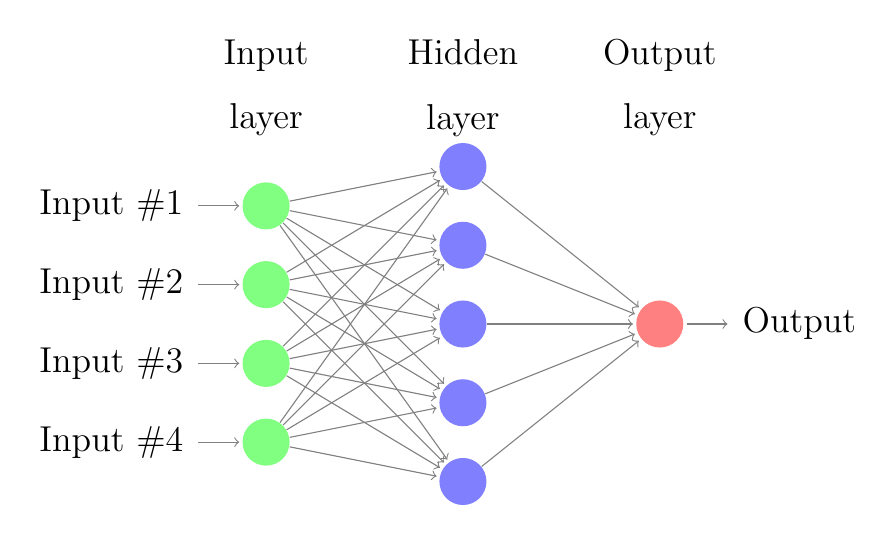
\begin{tikzpicture}[shorten >=1pt,->,draw=black!50, node distance=\layersep]
    \tikzstyle{every pin edge}=[<-,shorten <=1pt]
    \tikzstyle{neuron}=[circle,fill=black!25,minimum size=17pt,inner sep=0pt]
    \tikzstyle{input neuron}=[neuron, fill=green!50];
    \tikzstyle{output neuron}=[neuron, fill=red!50];
    \tikzstyle{hidden neuron}=[neuron, fill=blue!50];
    \tikzstyle{annot} = [text width=4em, text centered]

    % Draw the input layer nodes
    \foreach \name / \y in {1,...,4}
    % This is the same as writing \foreach \name / \y in {1/1,2/2,3/3,4/4}
        \node[input neuron, pin=left:Input \#\y] (I-\name) at (0,-\y) {};

    % Draw the hidden layer nodes
    \foreach \name / \y in {1,...,5}
        \path[yshift=0.5cm]
            node[hidden neuron] (H-\name) at (\layersep,-\y cm) {};

    % Draw the output layer node
    \node[output neuron,pin={[pin edge={->}]right:Output}, right of=H-3] (O) {};

    % Connect every node in the input layer with every node in the
    % hidden layer.
    \foreach \source in {1,...,4}
        \foreach \dest in {1,...,5}
            \path (I-\source) edge (H-\dest);

    % Connect every node in the hidden layer with the output layer
    \foreach \source in {1,...,5}
        \path (H-\source) edge (O);

    % Annotate the layers
    \node[annot,above of=H-1, node distance=1cm] (hl) {Hidden layer};
    \node[annot,left of=hl] {Input layer};
    \node[annot,right of=hl] {Output layer};
\end{tikzpicture}
%\caption{Artificial neural network}
\centering
\caption{Shallow neural networks with one hidden layer}
\end{figure}
ANN has drawn attention from well testing researchers since the 1990s. An early application in well testing was introduced by Al-Kaabi and Lee (1990) to identify the interpretation models from derivative plots. Juniardi and Ershaghi (1993) studied the complexities of using ANN with a focus on well test analysis of faulted reservoirs, and discussed some of the shortcomings of the ANN method. Around the same time, Ershaghi et al. (1993) proposed an enhanced approach based on the work of Al-Kaabi and Lee (1990), by training multiple ANNs where each neural net was designed to learn the patterns for a specific reservoir model. In 1995, Athichanagorn and Horne combined ANN with sequential predictive probability method to improve the accuracy of interpretation. ANN was used to generate initial parameter estimates of the candidate reservoir models that it identified. The candidate models and initial estimates were then passed to the sequential predictive probability method for final evaluations.

\subsection{Deep feed-foward networks}
Deep feed-forward networks, also called feed-forward neural networks, or multilayer perceptron (MLPS), are the quintessential learning models. The goal of a feedforward networks is to approximate some function f. For example, for a classifier, $y = f(x)$ maps an in put $\textbf{x}$ to a category y. A feed-forward networks defines a mapping $\mathbf{y} = f(\mathbf{x},\mathbf{\theta})$ and learns the values of parameters $\mathbf{\theta}$ that the result in the best function approximation.\cite{Ian}

\begin{figure}[H]
\centering
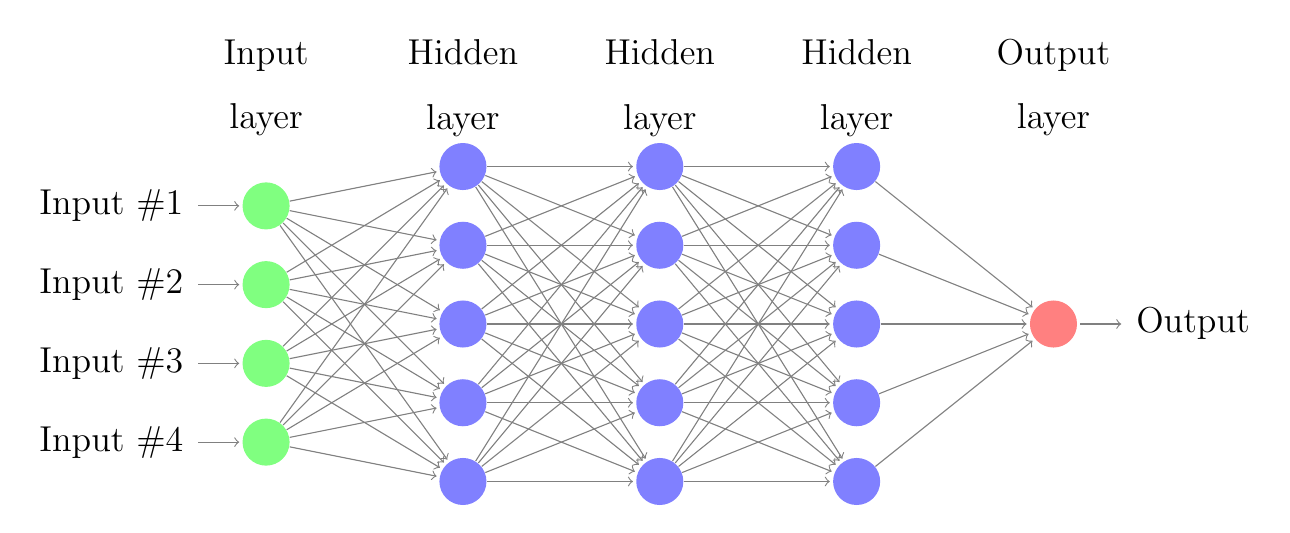
\begin{tikzpicture}[shorten >=1pt,->,draw=black!50, node distance=\layersep]
    \tikzstyle{every pin edge}=[<-,shorten <=1pt]
    \tikzstyle{neuron}=[circle,fill=black!25,minimum size=17pt,inner sep=0pt]
    \tikzstyle{input neuron}=[neuron, fill=green!50];
    \tikzstyle{output neuron}=[neuron, fill=red!50];
    \tikzstyle{hidden neuron1}=[neuron, fill=blue!50];
    \tikzstyle{hidden neuron2}=[neuron, fill=blue!50];
    \tikzstyle{hidden neuron3}=[neuron, fill=blue!50];
    \tikzstyle{annot} = [text width=4em, text centered]

    % Draw the input layer nodes
    \foreach \name / \y in {1,...,4}
    % This is the same as writing \foreach \name / \y in {1/1,2/2,3/3,4/4}
        \node[input neuron, pin=left:Input \#\y] (I-\name) at (0,-\y) {};

    % Draw the hidden layer nodes
    \foreach \name / \y in {1,...,5}
        \path[yshift=0.5cm]
            node[hidden neuron1] (H1-\name) at (\layersep,-\y cm) {};

    \foreach \name / \y in {1,...,5}
        \path[yshift=0.5cm]
            node[hidden neuron2] (H2-\name) at (\layersep +\layersep,-\y cm) {};

    \foreach \name / \y in {1,...,5}
        \path[yshift=0.5cm]
            node[hidden neuron3] (H3-\name) at (\layersep+\layersep+\layersep,-\y cm) {};
    % Draw the output layer node
    \node[output neuron,pin={[pin edge={->}]right:Output}, right of=H3-3] (O) {};

    % Connect every node in the input layer with every node in the
    % hidden layer.
    \foreach \source in {1,...,4}
        \foreach \dest in {1,...,5}
            \path (I-\source) edge (H1-\dest);
    \foreach \source in {1,...,5}
        \foreach \dest in {1,...,5}
            \path (H1-\source) edge (H2-\dest);
    \foreach \source in {1,...,5}
        \foreach \dest in {1,...,5}
            \path (H2-\source) edge (H3-\dest);
    % Connect every node in the hidden layer with the output layer
    \foreach \source in {1,...,5}
        \path (H3-\source) edge (O);

    % Annotate the layers
    \node[annot,above of=H1-1, node distance=1cm] (hl1) {Hidden layer};
    \node[annot,above of=H2-1, node distance=1cm] (hl2) {Hidden layer};
    \node[annot,above of=H3-1, node distance=1cm] (hl3) {Hidden layer};
    \node[annot,left of=hl1] {Input layer};
    \node[annot,right of=hl3] {Output layer};
\end{tikzpicture}
\caption{Deep feed forward neural networks}
\end{figure}
Recently, deep feed forward neural networks (or deep neural networks) has been applied widely in oil and gas industry. A new approach to reservoir characterization using deep neural netwokrs has been introduced by M. Korjani, Andrei Popa, Eli Grijalva, and Steve Cassidy \cite{example1}; well bore stability prediction \cite{example2}; deep recurrent neural network for surface pressure response during the hydraulics fracturing process \cite{example3}; deep neural network based prediction of leak-off pressure in offshore Norway \cite{example4}; New method for extracting the work status in Shipyard using Deep Neural Networks \cite{example5}; diagnostics of rod pumps with use of deep neural networks \cite{example7}; automatic salt-body classification using a deep convolutional neural network \cite{example8}; seismic problems has been issued by deep neural networks in various papers such as: deep neural network architectures arising in seismic inverse problems\cite{example6}; Application of convolutional and deep neural networks for GPU based seismic interpretations \cite{example9}. Beside, deep convolutional neural networks has also been built for geology problems: deep learning convolutional neural networks to predict porous media properties \cite{example10}, visual explanations from convolutional neural networks for fault detection\cite{example11}.

%\subsubsection{Restricted Boltzmann Machines}
%\subsubsection{Convolutional neural networks}
%Convolutional neural networks (CNNs, or ConvNets) are essential tools for deep learning, and are especially suited for analyzing image data. For example, you can use CNNs to classify images. To predict continuous data, such as angles and distances, you can include a regression layer at the end of the network.
\subsection{Simple Recurrent neural networks}
Recurrent neural networks (RNNs) exploit characteristics of a feedback network, allowing the model to construct a sequential representation of input data. However, simple RNNs have been notoriously difficult to train, due to their iterative nature and the highly volatile relationship between the parameters and the hidden states \cite{Bengio}.\\
The network is given a sequence of inputs. Then, the network computes a sequence of hidden states and a sequence of predictions for each step in time. The sequences are computed by iterating through a series of equations that updates the model’s weight matrices, hidden layers, and the output units. The RNN utilizes predefined vector-valued functions that contain a computable Jacobian and are typically non-linear and applied coordinate-wise\cite{Mar}.
\begin{figure}[H]
  \centering
  \fbox{\includegraphics[scale=0.25]{Fig/RNN.png}}
  \caption{Recurrent neural network simple architecture\cite{LSTM}}
\end{figure}

\subsection{Long short term memory}
Long short-term memory (LSTM) units (or blocks) are a building unit for layers of a recurrent neural network (RNN). A RNN composed of LSTM units is often called an LSTM network. A common LSTM unit is composed of a cell, an input gate, an output gate and a forget gate. The cell is responsible for "remembering" values over arbitrary time intervals; hence the word "memory" in LSTM. Each of the three gates can be thought of as a "conventional" artificial neuron, as in a multi-layer (or feedforward) neural network: that is, they compute an activation (using an activation function) of a weighted sum. Intuitively, they can be thought as regulators of the flow of values that goes through the connections of the LSTM; hence the denotation gate and there are connections between these gates and the cell. A detailed explanation has been introduced by Colah in his blogs about long short term memory\cite{LSTM}.
\begin{figure}[H]
    \centering
    \fbox{\includegraphics[scale=0.5]{Fig/LSTM.png}}
    \caption{Simple stretch of long short term memory\cite{LSTM}}
\end{figure}


\subsection{Gated Recurrent Unit}
In simple words, the GRU unit does not have to use a memory unit to control the flow of information like the LSTM unit. It can directly makes use of the all hidden states without any control. GRUs have fewer parameters and thus may train a bit faster or need less data to generalize. But, with large data, the LSTMs with higher expressiveness may lead to better results.\\
They are almost similar to LSTMs except that they have two gates: reset gate and update gate. Reset gate determines how to combine new input to previous memory and update gate determines how much of the previous state to keep. Update gate in GRU is what input gate and forget gate were in LSTM. We don't have the second non linearity in GRU before calculating the output, neither they have the output gate.
\begin{figure}[H]
  \centering
  \fbox{\includegraphics[scale=0.7]{Fig/GRU.png}}
  \caption{Simple stretch of Gated Recurrent Unit\cite{LSTM}}
\end{figure}





\clearpage

\chapter{Methodology}
\section{Input data}
The production dataset used in this paper is from Volve field on Norwegian continental shelf with around 8 years history. Daily oil, gas and water production data are all recorded consist with pressure, temperature and choke size as operation constraint. These production data are the main input variables for the machine learning and deep learning model, and it gives multi-phase production predictions in the future as model output.\\
In this research, bottom hole pressure (BHP), tubing head pressure (THP), bottom hole temperature (BHT), well head temperature (WHT), different pressure in casing (DP), choke size (CS) in percentage is the input for training machine learning and deep learning algorithms.
\begin{table}[H]
\caption{Description of data set}
\centering
\begin{adjustbox}{width=1\textwidth}
\small
\begin{tabular}{|c|c|c|c|c|c|c|c|c|c|}
\hline
\textbf{}      & \textbf{BHP} & \textbf{BHT} & \textbf{DP} & \textbf{CS} & \textbf{WHP} & \textbf{WHT} & \textbf{OIL} & \textbf{GAS} & \textbf{WATER} \\ \hline
\textbf{Count} & 2365.0       & 2365.0       & 2365.0      & 2365.0      & 2365.0       & 2365.0       & 2365.0       & 2365.0       & 2365.0         \\ \hline
\textbf{Mean}  & 249.09       & 102.09       & 209.74      & 78.48       & 39.36        & 82.10        & 1217.04      & 180380.41    & 2968.53        \\ \hline
\textbf{Std}   & 14.47        & 3.35         & 22.44       & 24.82       & 12.61        & 2.23         & 1052.86      & 149356.18    & 934.56         \\ \hline
\textbf{Min}   & 135.63       & 54.64        & 103.14      & 20.30       & 27.19        & 72.14        & 100.33       & 5928.54      & 100.16         \\ \hline
\textbf{25\%}  & 241.72       & 99.73        & 197.39      & 55.85       & 31.28        & 84.48        & 322.41       & 49848.46     & 2694.0         \\ \hline
\textbf{50\%}  & 247.56       & 101.14       & 208.75      & 97.92       & 32.84        & 87.20        & 950.38       & 151088.07    & 3203.3         \\ \hline
\textbf{75\%}  & 261.78       & 105.05       & 230.24      & 100.0       & 42.23        & 88.63        & 1876.97      & 285954.06    & 3541.83        \\ \hline
\textbf{Max}   & 281.31       & 106.77       & 239.84      & 100.0       & 115.06       & 93.51        & 5644.37      & 786328.36    & 5691.77        \\ \hline
\end{tabular}
\end{adjustbox}
\end{table}
\section{Work-flow}

\begin{figure}[H]
\centering
\includegraphics[scale=0.8]{Fig/3.png}
\caption{Work flow for using machine and deep learning algorithms}
\end{figure}

Almost every machine learning and deep learning algorithm has followed this work-flow above. First, all raw data need to be collected altogether. Feature engineering means the process of using domain knowledge of the data to create features that make machine learning algorithms work. Feature engineering is an informal topic, but it is considered essential in applied machine learning\cite{feature}. From Andrew Ng, a famous Professor in AI : "Applied machine learning is basically feature engineering".Feature engineering in this research consists of three step from preprocessing to cross-validation (CV) strategies and feature scaling. Machine learning models are implemented with Scikit-learn library, and deep learning models are also implemented with Keras library, two of these very useful and popular libraries for working with ML/DL algorithms.

\begin{figure}[H]
\centering
\includegraphics[scale=0.55]{Fig/4.png}
\caption{Detailed work flow for using machine learning and deep learning algorithms}
\end{figure}
\subsection{Gather data}
The process of gathering data depends on the type of problems that need to solve. In this thesis, raw production data are gathered in excel file include 24 columns data and each column represents specific type of data. Due to the mess of data include missing and noisy data, before applying any machine learning and deep learning methods, data need to be applied feature engineering in order to get clean and useful data.

\subsection{Data preprocessing}
Data preprocessing is a processing of cleaning the raw data into clean data. Some type of missing data, noisy data and inconsistent data need to be through a filter which is usually called "Feature Extraction" or feature engineering. In this thesis, even though there are 24 columns of raw data, almost of them is text data that give information about the type, ID, well-bore code and filed name data and other unusefull data for applying ML/DL algorithms. Another important aspect is outlier of the data. There are some error data that might be present in the dataset that deviated significantly other from observed data. So, this kind of data also need to be eliminated.
\subsection{Cross validation strategies}
There are two scenarios of cross-validation (CV) strategies have been built in this research. In first scenario, data is divided in three parts: training data (70\%), validation data (15\%) and test data (15\%) with suffering all (figure 7). In the second scenario, data is separated in to 5 different folds (figure 8) and algorithms will train and test alternatively in training and testing data in very loop.
\subsection{Feature scaling}
Feature scaling is a method used to normalize the range of independent variables or features of data. In data processing, it is also known as data normalization and is generally performed during the data preprocessing step. In this thesis, three ways feature scaling have been used:\\
\textbf{Normalization}
	\begin{equation}
	x' = \frac{x - average(x)}{max(x) - min(x)}
	\end{equation}
\textbf{Standardization} \\The result of standardization is that the features will be rescaled so that they will have the properties of a standard normal distribution with $\mu = 0 \& \sigma = 1$.
	\begin{equation}
	x' = \frac{x - \overline{x}}{\sigma}
	\end{equation}
where $\mu$ is the mean (average) and $\sigma$ is the standard deviation.\\
\textbf{Min-max scaling}
	\begin{equation}
	x' = \frac{x - min(x)}{max(x) - min(x)}
	\end{equation}
Min-max scaling have been chosen due to the reasons of unchangeable distribution of the data and better results compare with other methods.
\subsection{Machine learning and deep learning algorithms}
As shown in the Figure 4.2, a typical loop of using machine learning and deep learning algorithms is from initializing model to optimize, validate, testing and forecasting. Each of these steps have its specific definition and methods.
\begin{enumerate}
	\item Initialize model means setting all parameters of model to specific values. There are two popular ways is initialize all parameters to zero or to random values from standard normal distribution or uniform distribution and multiply it by a scalar such as 10.
	\item Optimize model means finding the best combination of hyperparameters of models for the purpose of getting the best result. During the training process, manual tunning and grid search are used for finding the best combination of hyperparameters of algorithms. There is a loop between optimizing and validate model means that repeating the procedure until reaching the desired accuracy score.
	\item Validate and testing model are referred to as the processing where a trained model is evaluated with a validation and testing dataset. They are aimed to find the optimal model with the best performance. There are a number of statical metrics that can be used for validating the results. Mean square error, maximum absolute error, coefficient of determination and person correlation have been used.
	\item After completing all previous steps above, the model can have ability to forecast. In this study, production rate include oil rate, gas rate, and water rate are the outputs from the training model.
\end{enumerate}

\chapter{Result and Discussion}
\section{Machine learning}
The the table bellow we show the result of every algorithm we have used. Coefficient of determination $(R^2)$ and mean squared error (MSE) have been used to evaluation algorithm.
\begin{align*}
R^{2}(y,\hat y) = 1 - \frac{\sum_{i = 1}^{n} (y_{i} - \hat y_{i})^2}{\sum_{i = 1}^{n} (y_{i} - \bar y)^2} \\
MSE(y,\hat y) = \frac{1}{n}\sum_{i=1}^{n}(y_{i} - \hat y_{i})^2
\end{align*}
Pearson correlation is also used for testing the model.
\begin{align*}
\rho_{X,Y} = \frac{cov(X,Y)}{\sigma_{X}\sigma_{Y}}
\end{align*}

\begin{table}[H]
\centering
\caption{Score and error of machine learning algorithms on oil}
\begin{adjustbox}{width=1\textwidth}
\small
\begin{tabular}{|l|c|c|c|c|c|}
\hline
\textbf{No} & \textbf{Model} & \textbf{Validation Score} & \textbf{Validation Error} & \textbf{Test Score} & \textbf{Test Error} \\ \hline
1           & Linear Regression                        & 0.82132                                             & 0.00598                                             & 0.80275                                       & 0.00609                                       \\ \hline
2           & Ridge                                    & 0.8257                                              & 0.00583                                             & 0.78125                                       & 0.00676                                       \\ \hline
3           & KNeighbors Regression                    & 0.9218                                              & 0.00262                                             & 0.95795                                       & 0.00130                                       \\ \hline
4           & Support Vector Regression                & 0.8556                                              & 0.00483                                             & 0.84564                                       & 0.00477                                       \\ \hline
5           & Decision Tree Regression                 & 0.94392                                             & 0.001876                                            & 0.95973                                       & 0.00124                                       \\ \hline
6           & Random Forest Regression                 & 0.9687                                              & 0.00138                                             & 0.9585                                        & 0.00128                                       \\ \hline
7           & Extra Tree Regression                    & 0.9569                                              & 0.00144                                             & 0.96031                                       & 0.00123                                       \\ \hline
8           & AdaBoost Regression                      & 0.90031                                             & 0.00334                                             & 0.90247                                       & 0.00301                                       \\ \hline
9           & Gradient Boosting Regression             & 0.9554                                              & 0.00149                                             & 0.9597                                        & 0.00124                                       \\ \hline
10          & XgBoost Regression                       & 0.92087                                             & 0.00265                                             & 0.93438                                       & 0.00203                                       \\ \hline
11          & LightGBM Regression                      & 0.89392                                             & 0.00355                                             & 0.93392                                       & 0.00204                                       \\ \hline
\end{tabular}
\end{adjustbox}
\end{table}
%\vspace{-100mm}
After comparing the result on validation and test set, we just picked up five algorithms that yield the best score on test set. Score and error of gas and water prediction can be found in appendix (table 10 and 11).
In order to evaluate how possible the algorithms can be applied to forecast a new set of data, we use the Pearson correlation for evaluation. The table below shows the Pearson correlation for the best five algorithms.
\begin{table}[h]
\caption{Pearson correlation of best five algorithms}
\centering
\begin{adjustbox}{width=1\textwidth}
\small
\begin{tabular}{|c|c|c|c|c|}
\hline
\textbf{No} & \textbf{Model}            & \textbf{Pearson correlation (oil)} & \textbf{Pearson correlation (gas)} & \textbf{Pearson correlation (water)} \\ \hline
1           & Extreme Gradient Boosting & 0.96667                            & 0.96895                            & 0.8988                               \\ \hline
2           & Decision Tree Regression  & 0.9798                             & 0.9596                             & 0.8970                               \\ \hline
3           & Random Forest Regression  & 0.97927                            & 0.9757                             & 0.9161                               \\ \hline
4           & Gradient Boosting Machine & 0.96689                            & 0.9745                             & 0.92                                 \\ \hline
5           & Extra Tree Regression     & 0.98065                            & 0.98205                            & 0.9351                               \\ \hline
\end{tabular}
\end{adjustbox}
\end{table}



\begin{figure}[H]
      \begin{minipage}[h]{1.0\linewidth}
         \centering
         \includegraphics[width=\linewidth]{MLs/oil}
      \end{minipage}
\vspace{0.00mm}
     \begin{minipage}[h]{1\linewidth}
        \centering
        \includegraphics[width=\linewidth]{MLs/gas}
      \end{minipage}
\hspace{0.00mm}
     \begin{minipage}[h]{1\linewidth}
        \centering
        \includegraphics[width=\linewidth]{MLs/water}
     \end{minipage}
\caption{Production rate prediction versus actual values}
\label{fig:furt}
\end{figure}



\begin{figure}[H]
     \begin{center}
%
		\subfigure[Extreme gradient boosting regression]{%
            \label{fig:fourth}
            \includegraphics[width=0.45\textwidth]{cv_oil/cv_xgb}
        }%
        \subfigure[Extra trees regression]{%
           \label{fig:second}
           \includegraphics[width=0.45\textwidth]{cv_oil/cv_ett}
        }\\ %  ------- End of the first row ----------------------%
        \subfigure[Light GBM regression]{%
            \label{fig:third}
            \includegraphics[width=0.45\textwidth]{cv_oil/cv_lgb}
        }%
        \subfigure[Random forest regression]{%
            \label{fig:fourth}
            \includegraphics[width=0.45\textwidth]{cv_oil/cv_rf}
        }

    \end{center}
    \caption{%
        Oil prediction using time series cross-validation method.
     }%
   \label{fig:subfigures}
\end{figure}


\begin{figure}[H]
     \begin{center}
%
		\subfigure[Extreme gradient boosting regression]{%
            \label{fig:fourth}
            \includegraphics[width=0.45\textwidth]{cv_gas/cv_gas_xgb}
        }%
        \subfigure[Extra trees regression]{%
           \label{fig:second}
           \includegraphics[width=0.45\textwidth]{cv_gas/cv_gas_ett}
        }\\ %  ------- End of the first row ----------------------%
        \subfigure[Light GBM regression]{%
            \label{fig:third}
            \includegraphics[width=0.45\textwidth]{cv_gas/cv_gas_lgb}
        }%
        \subfigure[Random forest regression]{%
            \label{fig:fourth}
            \includegraphics[width=0.45\textwidth]{cv_gas/cv_gas_rf}
        }
    \end{center}
    \caption{%
        Gas prediction using time series cross-validation method.
     }%
   \label{fig:subfigures}
\end{figure}
With all machine learning algorithms we have used, data need to be shuffled before training, the dependence of production rate followed time have vanished. Therefore, we continue to use time series cross-validation strategy on the same data set. Instead of using gradient boosting machine regressor, authors used LGBM and XGB algorithms because these algorithms have better result compare with GBM. Figure 5.2 and 5.3 have shown result of using time series cross-validation method on oil and water. There is a gap between actual values and prediction demonstrate the algorithms are not sufficient for time series prediction. Decision tree and random forest regression give better result compare with other algorithms.


\section{Deep learning}
Neural networks have been used widely in oil and gas industry since the time it is created. Compare with other machine learning algorithms, NNs have given better or worse result depend on the process of training. While shallow neural networks with one hidden layer (25 nodes) give lower score and error is bigger, deep neural networks with three hidden layers have increased the score and reduce error.\\
In this research, hyperparameters of neural networks are tuned (table 8) to find the best combination of them for giving a good result on the validation test. Moreover, we have used some very novel technique in AI, dropout and ReLU activation function, to train our neural networks. 
\subsection{Neural networks}
\begin{table}[H]
\caption{Score and error on oil prediction}
\centering
\begin{adjustbox}{width=1\textwidth}
\small
\begin{tabular}{|l|c|c|c|c|c|}
\hline
\textbf{No} & \textbf{Model}          & \textbf{Validation Score} & \textbf{Validation Error} & \textbf{Test Score} & \textbf{Test Error}  \\ \hline
1           & Shallow neural networks & 0.8563                        & 0.0048                    & 0.8426                  & 0.00486                                     \\ \hline
2           & Deep neural networks    & 0.9492                        & 0.001568                  & 0.94                    & 0.00199                                    \\ \hline
\end{tabular}
\end{adjustbox}
\end{table}

\begin{table}[H]
\caption{Score and error on gas prediction}
\centering
\begin{adjustbox}{width=1\textwidth}
\small
\begin{tabular}{|c|c|c|c|c|c|}
\hline
\textbf{No} & \textbf{Model}          & \textbf{Validation Score} & \textbf{Validation Error} & \textbf{Test Score} & \textbf{Test Error} \\ \hline
1           & Shallow Neural Networks & 0.6826                    & 0.0101                    & 0.6068              & 0.00948             \\ \hline
2           & Deep Neural Networks    & 0.7824                    & 0.00551                   & 0.7767              & 0.00574             \\ \hline
\end{tabular}
\end{adjustbox}
\end{table}


\begin{table}[H]
\caption{Score and error on water prediction}
\centering
\begin{adjustbox}{width=1\textwidth}
\small
\begin{tabular}{|c|c|c|c|c|c|}
\hline
\textbf{No} & \textbf{Model}          & \textbf{Validation Score} & \textbf{Validation Error} & \textbf{Test Score} & \textbf{Test Error} \\ \hline
1           & Shallow Neural Networks & 0.6826                    & 0.0101                    & 0.6068              & 0.00948             \\ \hline
2           & Deep Neural Networks    & 0.7824                    & 0.00551                   & 0.7767              & 0.00574             \\ \hline
\end{tabular}
\end{adjustbox}
\end{table}



\begin{table}[H]
\caption{Pearson correlation of neural networks}
\centering
\begin{adjustbox}{width=1\textwidth}
\small
\begin{tabular}{|c|c|c|c|c|}
\hline
\textbf{No} & \textbf{Model}          & \textbf{Pearson correlation (oil)} & \textbf{Pearson correlation (gas)} & \textbf{Pearson correlation (water)} \\ \hline
1           & Shallow Neural Networks & 0.9225                             & 0.9372                             & 0.8314                               \\ \hline
2           & Deep Neural Networks    & 0.9798                             & 0.9711                             & 0.9014                               \\ \hline
\end{tabular}
\end{adjustbox}
\end{table}

By plotting the actual and predicted values in one figure, a clear improvement of using deep neural networks has shown below:
\begin{figure}[H]
     \begin{center}
%
        \subfigure[Oil prediction]{%
            \label{fig:first}
            \includegraphics[width=0.32\textwidth]{NNs/oil_shallow}
        }%
        \subfigure[Gas prediction]{%
           \label{fig:second}
           \includegraphics[width=0.32\textwidth]{NNs/gas_shallow}
        }%  ------- End of the first row ----------------------%
        \subfigure[Water prediction]{%
            \label{fig:third}
            \includegraphics[width=0.32\textwidth]{NNs/water_shallow}
        }
    \end{center}
    \caption{%
        Production rate prediction using shallow neural networks.
     }%
   \label{fig:subfigures}
\end{figure}

\begin{figure}[H]
     \begin{center}
%
        \subfigure[Oil prediction]{%
            \label{fig:first}
            \includegraphics[width=0.32\textwidth]{NNs/oil_deep}
        }%
        \subfigure[Gas prediction]{%
           \label{fig:second}
           \includegraphics[width=0.32\textwidth]{NNs/gas_deep}
        }%  ------- End of the first row ----------------------%
        \subfigure[Water prediction]{%
            \label{fig:third}
            \includegraphics[width=0.32\textwidth]{NNs/water_deep}
        }
    \end{center}
    \caption{%
        Production rate prediction using deep neural networks.
     }%
   \label{fig:subfigures}
\end{figure}
It is obvious that neural networks have given better results when increasing the number of hidden layers from 1 to 3. However, like other machine learning algorithms, data also need to be shuffled before training. That lead to the loss of temporal characteristic. It is the main problem of using machine learning algorithms include neural networks if data is shuffled. This problem can be solved by using the recurrent neural networks which has been proven to be one of the most successful algorithms of time-series problems.

\subsection{Recurrent Neural Networks}
Recurrent neural networks algorithms are very powerful with time-series data. Data set is split in three-part train, validation and final 2 years (15\%) is the test set. Compare with machine learning models, RNNs have improved remarkably when predicted in the last two year. From figure 5.6, 5.7 and 5.8 above when using Recurrent neural networks (LSTM, GRU, SimpleRNN), a very close matching between prediction and actual values. Since GRU and LSTM give the best results on oil prediction, SimpleRNN is better with water forecasting.

\begin{figure}[H]
     \begin{center}
%
        \subfigure[Oil prediction]{%
            \label{fig:first}
            \includegraphics[width=0.32\textwidth]{DLN/LSTM_oil1}
        }%
        \subfigure[Gas prediction]{%
           \label{fig:second}
           \includegraphics[width=0.32\textwidth]{DLN/LSTM_gas1}
        }%  ------- End of the first row ----------------------%
        \subfigure[Water prediction]{%
            \label{fig:third}
            \includegraphics[width=0.32\textwidth]{DLN/LSTM_water1}
        }
    \end{center}
    \caption{%
        Production rate prediction using long short term memory.
     }%
   \label{fig:subfigures}
\end{figure}



\begin{figure}[H]
     \begin{center}
%
        \subfigure[Oil prediction]{%
            \label{fig:first}
            \includegraphics[width=0.32\textwidth]{DLN/GRU_oil}
        }%
        \subfigure[Gas prediction]{%
           \label{fig:second}
           \includegraphics[width=0.32\textwidth]{DLN/GRU_gas}
        }%  ------- End of the first row ----------------------%
        \subfigure[Water prediction]{%
            \label{fig:third}
            \includegraphics[width=0.32\textwidth]{DLN/GRU_water}
        }
    \end{center}
    \caption{%
        Production rate prediction using gated recurrent unit.
     }%
   \label{fig:subfigures}
\end{figure}


\begin{figure}[H]
     \begin{center}
%
        \subfigure[Oil prediction]{%
            \label{fig:first}
            \includegraphics[width=0.32\textwidth]{DLN/RNN_oil}
        }%
        \subfigure[Gas prediction]{%
           \label{fig:second}
           \includegraphics[width=0.32\textwidth]{DLN/RNN_gas}
        }%  ------- End of the first row ----------------------%
        \subfigure[Water prediction]{%
            \label{fig:third}
            \includegraphics[width=0.32\textwidth]{DLN/RNN_water}
        }
    \end{center}
    \caption{%
        Production rate prediction using simple recurrent neural networks.
     }%
   \label{fig:subfigures}
\end{figure}
 



\section{Applied long short term memory as the best algorithms}
After a comparison of the result with different algorithms, recurrent neural networks seem to be the most appropriate for time series production prediction. Hence, Long short term memory has been chosen to be continued to train to compare with convention and reservoir modeling methods. 
\subsection{Comparison with DCA}

A production profile from 01/01/2015 to 07/12/2016 has been used for comparison between LSTM and DCA.
\begin{figure}[H]
  \centering
  \fbox{\includegraphics[scale=0.6]{Fig/Hisdca.png}}
  \caption{History production of well F14}
\end{figure}

Due to the limit of decline curve analysis methods, DCA is only used when the well is in a boundary-dominated flow condition. This means DCA is possible with F14 and F12 wells prediction and the F14 well is chosen for using decline curve analysis. There are four periods in use for creating decline curves. A comparison between conventional decline curve analysis and LSTM algorithms have shown in figure below:
\begin{figure}[H]
  \centering
  \fbox{\includegraphics[scale=0.5]{Fig_theo/DCA.png}}
  \caption{Comparison of actual values, LSTM and DCA}
\end{figure}

\begin{table}[H]
\caption{Decline (D) values and time periods}
\centering
\begin{tabular}{|c|c|c|c|c|}
\hline
                     & \textbf{DCA\_357} & \textbf{DCA\_360} & \textbf{DCA\_394} & \textbf{DCA\_705} \\ \hline
\textbf{Time (days)} & 357               & 360               & 394               & 705               \\ \hline
\textbf{D values}    & 0.00172           & 0.0017            & 0.0031            & 0.0021            \\ \hline
\end{tabular}
\end{table}
Percentage error is used for comparison. The relative error is defined by:
\begin{equation}
\delta = \frac{\Delta x}{x} = \frac{|x_{0} - x|}{x}
\end{equation}
where $\Delta x$ is absolute error. Percentage error is 100\% times to relative error.
\begin{table}[H]
\caption{Cumulative oil production comparison}
\centering
\begin{adjustbox}{width=1\textwidth}
\begin{tabular}{|c|c|c|c|c|c|c|}
\hline
                        & \multicolumn{1}{l|}{\textbf{Actual values}} & \textbf{DCA\_357} & \textbf{DCA\_360} & \textbf{DCA\_394} & \textbf{DCA\_705} & \multicolumn{1}{l|}{\textbf{LSTM}} \\ \hline
\textbf{Cumulative oil} & 101424.84                                   & 183504.591        & 130018.689        & 83019.914         & 171241.554        & 107553.954                         \\ \hline
\textbf{Error}          & 0\%                                         & 80.92\%          & 28.2\%            & 18.15\%           & 68.83\%           & 6.04\%                             \\ \hline
\end{tabular}
\end{adjustbox}
\end{table}
Ideally, the optimized error should be as small as possible and could not be excessed 10\%.
From the table below, LSTM algorithms (6.04\% of error) have outperformed decline curve analysis methods in predict cumulative oil production, moreover Figure 5.9 shows that while LSTM fluctuates near the end of production, it has been the closest curve with the actual curve compare with the other decline analysis curve.

\subsection{Comparison with Eclipse}

\subsubsection{Well F1}
\begin{figure}[H]
     \begin{center}
%
		\subfigure[Oil prediction]{%
            \label{fig:fourth}
            \includegraphics[width=0.8\textwidth]{comparison/F1_oil}
        }\\%
        \subfigure[Gas prediction ]{%
           \label{fig:second}
           \includegraphics[width=0.8\textwidth]{comparison/F1_gas}
        }\\ %  ------- End of the first row ----------------------%
        \subfigure[Water prediction]{%
            \label{fig:third}
            \includegraphics[width=0.8\textwidth]{comparison/F1_water}
        }
    \end{center}
    \caption{%
        Production prediction on well F1
     }%
   \label{fig:subfigures}
\end{figure}



\subsubsection{Well F11}
\begin{figure}[H]
     \begin{center}
%
		\subfigure[Oil prediction]{%
            \label{fig:fourth}
            \includegraphics[width=0.8\textwidth]{comparison/F11_oil}
        }\\%
        \subfigure[Gas prediction ]{%
           \label{fig:second}
           \includegraphics[width=0.8\textwidth]{comparison/F11_gas}
        }\\ %  ------- End of the first row ----------------------%
        \subfigure[Water prediction]{%
            \label{fig:third}
            \includegraphics[width=0.8\textwidth]{comparison/F11_water}
        }

    \end{center}
    \caption{%
        Production prediction on well F11
     }%
   \label{fig:subfigures}
\end{figure}

\subsubsection{Well F12}
\begin{figure}[H]
     \begin{center}
%
		\subfigure[Oil prediction]{%
            \label{fig:fourth}
            \includegraphics[width=0.8\textwidth]{comparison/F12_oil}
        }\\%
        \subfigure[Gas prediction ]{%
           \label{fig:second}
           \includegraphics[width=0.8\textwidth]{comparison/F12_gas}
        }\\ %  ------- End of the first row ----------------------%
        \subfigure[Water prediction]{%
            \label{fig:third}
            \includegraphics[width=0.8\textwidth]{comparison/F12_water}
        }

    \end{center}
    \caption{%
        Production prediction on well F12
     }%
   \label{fig:subfigures}
\end{figure}

\subsubsection{Well F14}
\begin{figure}[H]
     \begin{center}
%
		\subfigure[Oil prediction]{%
            \label{fig:fourth}
            \includegraphics[width=0.8\textwidth]{comparison/F14_oil}
        }\\%
        \subfigure[Gas prediction ]{%
           \label{fig:second}
           \includegraphics[width=0.8\textwidth]{comparison/F14_gas}
        }\\ %  ------- End of the first row ----------------------%
        \subfigure[Water prediction]{%
            \label{fig:third}
            \includegraphics[width=0.8\textwidth]{comparison/F14_water}
        }

    \end{center}
    \caption{%
        Production prediction on well F14
     }%
   \label{fig:subfigures}
\end{figure}


\subsubsection{Well F15}
\begin{figure}[H]
     \begin{center}
%
		\subfigure[Oil prediction]{%
            \label{fig:fourth}
            \includegraphics[width=0.8\textwidth]{comparison/F15_oil}
        }\\
        \subfigure[Gas prediction ]{%
           \label{fig:second}
           \includegraphics[width=0.8\textwidth]{comparison/F15_gas}
        }\\%  ------- End of the first row ----------------------%
        \subfigure[Water prediction]{%
            \label{fig:third}
            \includegraphics[width=0.8\textwidth]{comparison/F15_water}
        }

    \end{center}
    \caption{%
        Production prediction on well F15
     }%
   \label{fig:subfigures}
\end{figure}
Different from Eclipse simulator where an average of 10 days of production has been matched with actual values, using LSTM memory can predict each day during production period.\\
According to the five tables 5.11, 5.12, 5.13, 5.14 and 5.15 above, LSTM algorithm has given better results compared with Eclipse model in well F1, F14, and F15. As shown in the figures above, LSTM not only give a better matching with the actual values in these well, but also in prediction they are more likely to catch the trend of production in the future. However, in the well F11 and F12, Eclipse model has better matching. This might be the limit of LSTM algorithms because of the data noise.\\
Next, cumulative production will be compared between Eclipse output and LSTM. Oil rate will be chosen for this comparison in this study. Gas and water comparison can be found in the appendix for reference.

\begin{figure}[H]
  \centering
  \includegraphics[width=\linewidth]{Cumulative/F1}
  \caption{Cumulative oil production on F1}
\end{figure}

\begin{figure}[H]
  \centering
  \includegraphics[width=\linewidth]{Cumulative/F11}
  \caption{Cumulative oil production on F11}
\end{figure}

\begin{figure}[H]
  \centering
  \includegraphics[width=\linewidth]{Cumulative/F12}
  \caption{Cumulative oil production on F12}
\end{figure}


\begin{figure}[H]
  \centering
  \includegraphics[width=\linewidth]{Cumulative/F14}
  \caption{Cumulative oil production on F14}
\end{figure}

\begin{figure}[H]
  \centering
  \includegraphics[width=\linewidth]{Cumulative/F15}
  \caption{Cumulative oil production on F15}
\end{figure}

\begin{table}[H]
\caption{Cumulative oil production by well}
\centering
\begin{adjustbox}{width=1\textwidth}
\small
\begin{tabular}{|c|c|c|c|c|c|}
\hline
\textbf{}                                  & \textbf{Well F1} & \textbf{Well F11} & \textbf{Well F12} & \textbf{Well F14} & \textbf{Well F15} \\ \hline
\textbf{Actual cumulative production (m3)} & 177709.3         & 1227203           & 4579610           & 3942233           & 148518.6          \\ \hline
\textbf{Cumulative oil of LSTM (m3)}       & 181144.8         & 1224349           & 4912712           & 3960222           & 150325.6          \\ \hline
\textbf{Error (\%)}                        & 1.93             & 0.23              & 7.27\%            & 0.45              & 1.21              \\ \hline
\end{tabular}
\end{adjustbox}
\end{table}

On well F11 and F14, LSTM gives the prediction of cumulative oil production with 0.23\% and 0.45\% error respectively. On well F1 and F15, errors are 1.93\% and 1.21 and F12 well is 7.27\%. These errors are supposed to be acceptable for further using of LSTM algorithm.


\subsubsection{Total cumulative oil production in comparison}
\begin{figure}[H]
  \centering
  \includegraphics[width=\linewidth]{Cumulative/SS1}
  \caption{Total production by day from 2008 to 2016}
\end{figure}

\begin{figure}[H]
  \centering
  \includegraphics[width=\linewidth]{Cumulative/SS}
  \caption{Total cumulative oil production comparison}
\end{figure}

\begin{table}[H]
\caption{Total cumulative oil production and errors}
\centering
\begin{adjustbox}{width=1\textwidth}
\small
\begin{tabular}{|c|c|c|c|}
\hline
\textbf{}       & \textbf{Actual cumulative production} & \textbf{Cumulative oil of LSTM} & \textbf{Cumulative oil of Eclipse} \\ \hline
\textbf{Values} & 10037081                              & 1043256                         & 9980819                            \\ \hline
\textbf{Error(\%)}  & 0                                  & 3.94                          & 0.56                             \\ \hline
\end{tabular}
\end{adjustbox}
\end{table}
The Volve reservoir model produced 9980819 $m^{3}$ of oil for 3,197 days. The cumulative oil from historical production was 10037081 $m^{3}$. Long short term memory gives the output of 1043256 $m^{3}$, slightly greater than actual values due to the mismatch of well F12 (7.97
\% from table 5.9). Although the error given by LSTM is slightly bigger than reservoir model, it still a very good match of production rate.\\
In addition, compare with building a complex reservoir model, LSTM algorithms just cost less time and effort to construct. Since the objective is to study the potential of artificial intelligence in production prediction, it is practically to use AI in brown field which have a great amount of historical data. But in case of lack of data, we can use it as a tool for production optimization in a short period of time.


\chapter{Conclusion}
In this thesis, the author has applied some AI technique include machine and deep learning algorithms to predict the production rate of oil well in different scenarios. Different algorithms have been used and comparison between them have shown that while machine learning gain good result in the production phases with the shuffle, the recurrent neural networks have improved the prediction with .\\
The following conclusions from this study are:
\begin{itemize}
	\item The machine learning and deep learning algorithms used in the thesis significantly rely on the amount of data to develop the capacity of production prediction.
	\item The quality of prediction highly depends on the data input. If the input is messy and inconsistent, then the production prediction can be unreliable.
	\item Since machine learning have gained good result when the data is shuffled, hence in order to predict time series production rate, recurrent neural networks are performed. Machine learning algorithms can also be used for production optimization. The constraint conditions of producing well can be modified and regulated based on a complicated relationship that was acquired from using machine learning algorithms. 
	\item Compare with conventional decline curve analysis (Arps), LSTM has outperformed due to the ability in time-series prediction. In Volve field studies, LSTM is better than reservoir simulation (Eclipse) at well F14 and F15 and close to the accuracy of actual values in all five wells. It demonstrates the ability of using Artificial Intelligence in production forecasting.
	\item While reservoir modeling needs a great amount of time and efforts to construct a reservoir model with extensive domain knowledge of geology, geophysics, petrophysics, reservoir engineering, and reservoir simulation, LSTM only based the historical data to complete the tasks. So, in this circumstance LSTM is working on the cutting-edge methods, and need to be studied carefully in the future in order to give better results. 
\end{itemize}
Also, a work flow of using machine learning and deep learning algorithms has been built with detailed explanations.\\
This study has demonstrated that without domain knowledge in oil and gas industry and complicated physics-based modeling, Artificial Intelligent can help engineer in production forecasting in effective ways. AI has been proven their potential and could be useful tools in oil and gas industry.\\
Furthermore, in the next study, gas-oil ratio (GOR), water-cut, water gas ratio (WGR) and bottom hole pressure can be predicted.

\bibliographystyle{unsrt}  
\begin{thebibliography}{1}

\bibitem{Hedong}
Hedong Sun.
\newblock Advanced Production Decline Analysis and Application.
\newblock Gulf Professional Publishing (2015).

\bibitem{Tarek}
Tarek Ahmed.
\newblock Reservoir Engineerin Handbook - Fourth Edition.

\bibitem{His1}
Havard Johnsen Reitan
\newblock History Matching: Effekten av tilgjengelig informasjon.

\bibitem{His2}
James R. Gilman and Chet Ozgen (Society of Petroleum Engineers)
\newblock Reservoir Simulation: History Matching and Forecasting.

\bibitem{His3}
Williams, M.A., Keating, J.F., Barghouty, M.F.
\newblock The stratigraphic method: a structured approach to history-matching complex simulation models. SPE Reservoir Evaluation  Engineering 1(2),169–176 (1998).

\bibitem{His4}
Dean S.Oliver and Yan Chen.
\newblock Recent progress on reservoir history matching: a review.

\bibitem{Cao}
Cao, Q., Banerjee, R., Gupta, S., Li, J., Zhou, W., \& Jeyachandra, B. 2016.
\newblock Data Driven Production Forecasting Using Machine Learning
\newblock Presented at SPE Argentina Exploration and Production of Unconventional Resources Symposium, Buenos Aires, Argentina, 1-3 June.

\bibitem{Ristanto}
Tita Ristanto.
\newblock Machine Learning
applied To Multiphase Production Problems.
\newblock MS Thesis, Standford University, 2018.

\bibitem{Boomer}
Boomer, R.J. (1995).
\newblock Predicting Production Using a Neural Network (Artificial Intelligence Beats Human Intelligence).
\newblock Society of Petroleum Engineers (SPE 30202).

\bibitem{Suhag}
Suhag, A., Ranjith, R., and Aminzadeh, F. (2017).
\newblock Comparison of Shale Oil Production Fore- casting using Empirical Methods and Artificial Neural Networks.
\newblock University of Southern Cali- fornia. SPE ATCE (SPE-187112-MS).

\bibitem{Sun}
J. Sun, X. Ma, and M. Kazi (2018),CSE ICON.
\newblock Comparison of Decline Curve Analysis DCA with Recursive Neural Networks RNN for Production Forecast of Multiple Wells
\newblock SPE-190104-MS doi: \href{https://doi.org/10.2118/190104-MS}{SPE-190104-MS}

\bibitem{Al}
Al-Kaabi, A. U. and Lee, W.J. 1990.
\newblock Using Artificial Neural Networks to Identify the Well Test Interpretation Model.
\newblock Presented at the Petroleum Computer Conference, Denver, Colorado, 25-28 June. SPE-20332.

\bibitem{Bishop}
Christopher M. Bishop
\newblock Pattern Recognition and Machine Learning.
\newblock Linear Model page 138-139
 
\bibitem{Dom}
Dominique Guillot
\newblock Introduction to Data Mining and Analysis
Decision trees.
\newblock April 6, 2016.

\bibitem{Ho}
Ho, Tin Kam (1995).
\newblock Random Decision Forests (PDF).
\newblock Proceedings of the 3rd International Conference on Document Analysis and Recognition, Montreal, QC, 14–16 August 1995. pp. 278–282.

\bibitem{DO}
D. O. Hebb.
\newblock The Organization of Behavior: A Neuropsychological Approach.
\newblock John Wiley \& Sons, 1949.
 
\bibitem{Bengio}
Y.Bengio, P.Simard, and P.Frasconi.
\newblock Learning long-term dependencies with gradient descent is difficult.
\newblock Neural Networks, IEEE Transactions on 5, no. 2 (1994): 157-166.


\bibitem{Ian}
Ian Goodfellow and Yoshua Bengio and Aaron Courville.
\newblock Deeplearning text book.
\newblock An MIT press book.

\bibitem{Hastie}
Hastie, T. et al., (2001).
\newblock The Elements of Statistical Learning. Springer New York Inc., New York, NY, USA.

\bibitem{Extre}
Pierre Geurts and Damien Ernst and Louis Wehenkel.
\newblock Extremely randomized trees

\bibitem{Gradient}
Friedman, J.H. (2011). 
\newblock Greedy Function Approximation: A Gradient Boosting Machine. Annals of Statistics. JSTOR.

\bibitem{sklearn}
Sklearn Library.
\newblock Machine learning in Python
\newblock Journal of machine learning research, volume 12, 2825--2830, 2011.

\bibitem{xgboost}
Chen, Tianqi and Guestrin, Carlos.
\newblock XGBoost: A Scalable Tree Boosting System.
\newblock Proceedings of the 22nd ACM SIGKDD International Conference on Knowledge Discovery and Data Mining 2016.

\bibitem{light}
Guolin Ke, Qi Meng, Thomas Finley, Taifeng Wang, Wei Chen, Weidong Ma, Qiwei Ye, Tie-Yan Liu. \newblock "LightGBM: A Highly Efficient Gradient Boosting Decision Tree". 
\newblock Advances in Neural Information Processing Systems 30 (NIPS 2017), pp. 3149-3157.

\bibitem{Mar}
Martens, James, and IlyaSutskever.
\newblock Learning recurrent neuralnetworks with hessian-free optimization.
\newblock In Proceedings of the 28th International Conference on Machine Learning (ICML-11), pp. 1033-1040. 2011.

\bibitem{LSTM}
\href{https://colah.github.io/posts/2015-08-Understanding-LSTMs/}{Understanding LSTM Networks}

\bibitem{Volve}
\href{https://www.equinor.com/en/news/14jun2018-disclosing-volve-data.html}{Volve dataset by Equinor company}

\bibitem{feature}
\href{https://en.wikipedia.org/wiki/Feature_engineering}{Wikipedia feature engineering}

\bibitem{example1}
M. Korjani, Andrei Popa, Eli Grijalva, Steve Cassidy and I. Ershaghi.
\newblock A New Approach to Reservoir Characterization Using Deep Learning Neural Networks.

\bibitem{example2}
E. E. Okpo, A. Dosunmu, and B. S. Odagme, University of Port Harcourt
\newblock Artificial Neural Network Model for Predicting Wellbore Instability.

\bibitem{example3}
Srinath Madasu and Keshava P. Rangarajan, Halliburton
\newblock Deep Recurrent Neural Network DRNN Model for Real-Time Multistage Pumping Data.

\bibitem{example4}
Jung Chan Choi, Elin Skurtveit, and Lars Grande, NGI
\newblock Deep Neural Network Based Prediction of Leak-Off Pressure in Offshore Norway.

\bibitem{example5}
Tanaka, Takashi, Shinoda, Takeshi Kyushu University
\newblock A Method for Extracting the Work Status in Shipyard Using Deep Neural Networks.

\bibitem{example6}
Maarten V. de Hoop, Rice University
\newblock Deep neural network architectures arising in seismic inverse problems.

\bibitem{example7}
A.G. Mihajlov, S.S. Shubin, A.V. Alferov, R.N. Imashev, V.U. Yamaliev
\newblock Improvement of efficiency of diagnostics of rod pumps with use of deep neural networks.

\bibitem{example8}
Yunzhi Shi, Xinming Wu and Sergey Fome.
\newblock Automatic salt-body classification using a deep convolutional neural network.

\bibitem{example9}
Sarblund Haroon, Sergey Alyamkin, and Ramachandra Shenoy, AlphaX Decision Sciences LLC
\newblock Application of Convolutional and Deep Neural Networks for GPU Based Seismic Interpretations.

\bibitem{example10}
Naif Alqahtani, Ryan T.Armstrong, and Peyman Mostaghimi.

\newblock Deep Learning Convolutional Neural Networks to Predict Porous Media Properties.

\bibitem{example11}
Zhining Liu, Chenyung Song, Bin She, Kunhong Li, Xingmiao Yao, Guangmin Hu.
\newblock Visual explanations from convolutional neural networks for fault detection.


\end{thebibliography}


%\begin{appendices}
\appendix
\appendixheaderoff
\chapter{Preprocessing and data used in thesis}

\begin{figure}[H]
\minipage{0.5\textwidth}
  \includegraphics[width=\linewidth]{Preprocessing/1}
  \caption{Data before feature engineering}\label{fig:awesome_image1}
\endminipage\hfill
\minipage{0.5\textwidth}
  \includegraphics[width=\linewidth]{Preprocessing/2}
  \caption{Data after feature engineering}\label{fig:awesome_image2}
\endminipage\hfill
\end{figure}

%\begin{figure}[H]
%\minipage{0.5\textwidth}
  %\includegraphics[width=\linewidth]{Preprocessing/box}
  %\caption{Box plot of input}\label{fig:awesome_image1}
%\endminipage\hfill
%\minipage{0.5\textwidth}
  %\includegraphics[width=\linewidth]{Preprocessing/boxplot}
  %\caption{Box plot of production rate}\label{fig:awesome_image2}
%\endminipage\hfill
%\end{figure}


\begin{figure}[H]
  \centering
  \includegraphics[width=\linewidth]{Preprocessing/box}
  \caption{Box plot of input}
\end{figure}

\begin{figure}[H]
  \centering
  \includegraphics[width=\linewidth]{Preprocessing/boxplot}
  \caption{Box plot of production rate}
\end{figure}

\begin{figure}[H]
  \centering
  \includegraphics[width=\linewidth]{Preprocessing/corr1}
  \caption{Correlation maxtrix of variables}
\end{figure}


\begin{table}[H]
\caption{Sample data for applying machine learning and deep learning}
\centering
\begin{adjustbox}{width=1\textwidth}
\small
\begin{tabular}{@{}llllllllll@{}}
\toprule
\textbf{DATE} & \textbf{BHP} & \textbf{BHT} & \textbf{DP} & \textbf{CS(\%)} & \textbf{WHP} & \textbf{WHT} & \textbf{OIL} & \textbf{GAS} & \textbf{WAT} \\ \midrule
1/30/09       & 257.44       & 105.34       & 163.29      & 35.30           & 94.15        & 61.05        & 4535.43      & 649388.07    & 298.19       \\
2/11/09       & 261.48       & 105.36       & 164.35      & 34.70           & 97.13        & 65.80        & 4379.88      & 629307.34    & 143.54       \\
2/20/09       & 264.39       & 105.41       & 166.21      & 34.78           & 98.17        & 64.99        & 4509.07      & 638750.17    & 108.74       \\
2/22/09       & 266.71       & 105.40       & 166.27      & 34.05           & 100.44       & 67.33        & 4319.02      & 612912.62    & 106.60       \\
2/23/09       & 266.67       & 105.41       & 166.51      & 34.40           & 100.15       & 66.99        & 4417.66      & 625514.01    & 117.37       \\
2/25/09       & 269.71       & 105.36       & 166.93      & 31.05           & 102.78       & 69.95        & 3226.61      & 460948.01    & 118.99       \\
2/26/09       & 268.34       & 105.43       & 167.28      & 34.31           & 101.06       & 67.85        & 4411.90      & 628668.27    & 134.19       \\
2/27/09       & 268.75       & 105.44       & 167.40      & 34.31           & 101.35       & 68.19        & 4376.91      & 625510.25    & 152.76       \\
…             & …            & …            & …           & …               & …            & …            & …            & …            & …            \\
…             & …            & …            & …           & …               & …            & …            & …            & …            & …            \\
6/28/16       & 269.88       & 100.17       & 238.91      & 45.13           & 30.97        & 5.45         & 102.26       & 16444.37     & 2973.66      \\
6/29/16       & 269.83       & 100.19       & 238.94      & 45.20           & 30.89        & 5.37         & 102.38       & 16458.56     & 2980.12      \\
6/30/16       & 269.83       & 100.20       & 238.89      & 45.16           & 30.93        & 5.40         & 101.47       & 16397.18     & 2985.45      \\
7/1/16        & 269.89       & 100.20       & 238.91      & 45.16           & 30.98        & 5.32         & 102.89       & 16369.86     & 2979.13      \\
7/2/16        & 269.79       & 100.22       & 238.87      & 45.18           & 30.93        & 5.39         & 101.58       & 16365.91     & 2992.00      \\
7/3/16        & 269.79       & 100.23       & 238.83      & 45.11           & 30.96        & 5.44         & 102.43       & 16269.74     & 2976.87      \\
7/4/16        & 269.78       & 100.24       & 238.82      & 45.08           & 30.96        & 5.44         & 100.67       & 16263.02     & 2990.10      \\
7/5/16        & 269.77       & 100.25       & 238.80      & 45.08           & 30.97        & 5.43         & 101.88       & 16284.48     & 2974.30      \\
7/7/16        & 266.20       & 100.31       & 238.44      & 93.42           & 27.76        & 2.19         & 106.19       & 17427.78     & 3172.96      \\
7/8/16        & 266.04       & 100.33       & 238.47      & 100.00          & 27.56        & 2.00         & 106.30       & 17541.20     & 3187.95      \\
7/9/16        & 268.81       & 100.30       & 239.08      & 82.19           & 29.73        & 4.11         & 102.09       & 16681.29     & 2326.24      \\
7/10/16       & 265.92       & 100.34       & 238.40      & 100.00          & 27.52        & 1.96         & 113.38       & 18753.12     & 3185.47      \\
7/11/16       & 267.77       & 100.32       & 238.64      & 91.16           & 29.13        & 3.41         & 108.84       & 17979.28     & 3056.29      \\
7/12/16       & 266.00       & 100.35       & 238.27      & 100.00          & 27.73        & 1.94         & 113.84       & 18543.76     & 3148.91      \\ \bottomrule
\end{tabular}
\end{adjustbox}
\end{table}





\chapter{Hyperparametes optimization}

\begin{table}[H]
\caption{Hyperparametes to optimize machine learning algorithms}
\centering
\begin{adjustbox}{width=1\textwidth}
\small
\begin{tabular}{|c|c|c|}
\hline
\textbf{No} & \textbf{Model}               & \textbf{Hyperparametes}                                            \\ \hline
1           & Linear Regression            & Nomalization                                                       \\ \hline
2           & Ridge                        & alpha (0.05), solver('auto')                                       \\ \hline
3           & KNeighbors Regression        & n\_neighbors (3),                                                  \\ \hline
4           & Support Vector Regression    & kernel ('rbf), C (1e1) , gamma = 10                                \\ \hline
5           & Decision Tree Regression     & max\_depth (10)                                                    \\ \hline
6           & Random Forest Regression     & n\_estimators = 200, max\_depth (8),,max\_features('sqrt')         \\ \hline
7           & Extra Tree Regression        & n\_estimators=200, min\_samples\_split(25), min\_samples\_leaf(35) \\ \hline
8           & AdaBoost Regression          & n\_estimators = 50                                                 \\ \hline
9           & Gradient Boosting Regression & n\_estimators(300), learning\_rate (0.005),,max\_depth(4)          \\ \hline
10          & XgBoost Regression           & n\_estimators(220), learning\_rate(0.05), max\_depth(3)            \\ \hline
11          & LightGBM Regression          & n\_estimators(720), learning\_rate (0.05)                          \\ \hline
\end{tabular}
\end{adjustbox}
\end{table}

\begin{table}[H]
\caption{Hyperparameters to optimize  deep learning algorithms}
\centering
\begin{adjustbox}{width=1\textwidth}
\small
\begin{tabular}{|c|c|c|}
\hline
\textbf{No} & \textbf{Hyperparameters} & \textbf{Type}                         \\ \hline
1           & Activation function     & tanh, ReLU, sigmoid, linear           \\ \hline
2           & Dropout (for DNN)       & 0.1 - 0.9, 0.4 , 0.5                  \\ \hline
3           & Hidden layers (in NNs)  & 0 - 4                                 \\ \hline
4           & Hidden layer nodes      & 10 - 500, 8 ,20, 50                   \\ \hline
5           & Loss function           & MSE, MAE, RMSE                        \\ \hline
6           & Metrics                 & MAE, MSE                              \\ \hline
7           & Optimizer               & SGD, LBFGS, Adagrad, Adam, RMSProp    \\ \hline
8           & Momentum                & None, regular, Nesterov               \\ \hline
9           & Learning rate           & 0.0001, 0.001, 0.005, 0.01, 0.03, 0.3 \\ \hline
10          & Learning rate decay     & 0 - 1e-3, 1e-6                        \\ \hline
11          & Regularization          & None, L1, L2, EarlyStopping           \\ \hline
12          & Hyperparameters search   & GridSearch, GridsearchCV              \\ \hline
\end{tabular}
\end{adjustbox}
\end{table}





\chapter{Machine learning result}
\begin{table}[H]
\caption{Score and error of machine learning algorithms on gas production}
\centering
\begin{adjustbox}{width=1\textwidth}
\small
\begin{tabular}{|l|c|c|c|c|c|}
\hline
\textbf{No} & \textbf{Model}               & \textbf{Validation Score} & \textbf{Validation Error} & \textbf{Test Score} & \textbf{Test Error} \\ \hline
1           & Linear Regression            & 0.8539                    & 0.00577                   & 0.8011              & 0.00599             \\ \hline
2           & Ridge                        & 0.8187                    & 0.00619                   & 0.8477              & 0.0057              \\ \hline
3           & KNeighbors Regression        & 0.9323                    & 0.00231                   & 0.9741              & 0.000967            \\ \hline
4           & Support Vector Regression    & 0.8610                    & 0.00474                   & 0.8817              & 0.00442             \\ \hline
5           & Decision Tree Regression     & 0.9452                    & 0.00187                   & 0.9625              & 0.0014              \\ \hline
6           & Random Forest Regression     & 0.9652                    & 0.00155                   & 0.9545              & 0.0013              \\ \hline
7           & Extra Tree Regression        & 0.9506                    & 0.00168                   & 0.9821              & 0.00068             \\ \hline
8           & AdaBoost Regression          & 0.9056                    & 0.00322                   & 0.9195              & 0.00301             \\ \hline
9           & Gradient Boosting Regression & 0.9685                    & 0.00112                   & 0.9474              & 0.00188             \\ \hline
10          & XgBoost Regression           & 0.9256                    & 0.00253                   & 0.955               & 0.00168             \\ \hline
11          & LightGBM Regression          & 0.8980                    & 0.00355                   & 0.9496              & 0.00204             \\ \hline
\end{tabular}
\end{adjustbox}
\end{table}

\begin{table}[H]
\caption{Score and error of machine learning algorithms on water production}
\centering
\begin{adjustbox}{width=1\textwidth}
\small
\begin{tabular}{|l|c|c|c|c|c|}
\hline
\textbf{No} & \textbf{Model}               & \textbf{Validation Score} & \textbf{Validation Error} & \textbf{Test Score} & \textbf{Test Error} \\ \hline
1           & Linear Regression            & 0.6133                    & 0.0101                    & 0.5228              & 0.013               \\ \hline
2           & Ridge                        & 0.599                     & 0.0105                    & 0.523               & 0.013               \\ \hline
3           & KNeighbors Regression        & 0.9032                    & 0.00254                   & 0.8889              & 0.00303             \\ \hline
4           & Support Vector Regression    & 0.8501                    & 0.00394                   & 0.8387              & 0.00477             \\ \hline
5           & Decision Tree Regression     & 0.881                     & 0.00313                   & 0.7822              & 0.00595             \\ \hline
6           & Random Forest Regression     & 0.9197                    & 0.00211                   & 0.8904              & 0.00299             \\ \hline
7           & Extra Tree Regression        & 0.9057                    & 0.00248                   & 0.9015              & 0.00268             \\ \hline
8           & AdaBoost Regression          & 0.7418                    & 0.00679                   & 0.7473              & 0.0069              \\ \hline
9           & Gradient Boosting Regression & 0.9071                    & 0.00244                   & 0.9124              & 0.00239             \\ \hline
10          & XgBoost Regression           & 0.8819                    & 0.0031                    & 0.8856              & 0.00312             \\ \hline
11          & LightGBM Regression          & 0.8481                    & 0.00399                   & 0.8591              & 0.00385             \\ \hline
\end{tabular}
\end{adjustbox}
\end{table}

\begin{figure}[H]
\centering
\includegraphics[width=.3\textwidth]{5best_oil/DCT}\quad
\includegraphics[width=.3\textwidth]{5best_oil/ETT}\quad
\includegraphics[width=.3\textwidth]{5best_oil/GBM}

\medskip

\includegraphics[width=.3\textwidth]{5best_oil/RF}\quad
\includegraphics[width=.3\textwidth]{5best_oil/XGB}

\caption{Best five  model on oil prediction}
\label{pics:blablabla}
\end{figure}

\begin{figure}[H]
\centering
\includegraphics[width=.3\textwidth]{5best_gas/DCT}\quad
\includegraphics[width=.3\textwidth]{5best_gas/ETT}\quad
\includegraphics[width=.3\textwidth]{5best_gas/GBM}

\medskip

\includegraphics[width=.3\textwidth]{5best_gas/RF}\quad
\includegraphics[width=.3\textwidth]{5best_gas/XGB}

\caption{Best five model on gas prediction}
\label{pics:blablabla}
\end{figure}
\begin{figure}[H]
\centering
\includegraphics[width=.3\textwidth]{5best_water/DCT}\quad
\includegraphics[width=.3\textwidth]{5best_water/ETT}\quad
\includegraphics[width=.3\textwidth]{5best_water/GBM}

\medskip

\includegraphics[width=.3\textwidth]{5best_water/RF}\quad
\includegraphics[width=.3\textwidth]{5best_water/XGB}

\caption{Best five model on water predict}
\label{pics:blablabla}
\end{figure}
\begin{figure}[H]
     \begin{center}
%
		\subfigure[Extreme gradient boosting regression]{%
            \label{fig:fourth}
            \includegraphics[width=0.45\textwidth]{cv_water/water_xgb}
        }%
        \subfigure[Extra trees regression]{%
           \label{fig:second}
           \includegraphics[width=0.45\textwidth]{cv_water/water_ett}
        }\\ %  ------- End of the first row ----------------------%
        \subfigure[Light GBM regression]{%
            \label{fig:third}
            \includegraphics[width=0.45\textwidth]{cv_water/water_lgb}
        }%
        \subfigure[Random forest regression]{%
            \label{fig:fourth}
            \includegraphics[width=0.45\textwidth]{cv_water/water_rf}
        }

    \end{center}
    \caption{%
        Water prediction using time series cross-validation method.
     }%
   \label{fig:subfigures}
\end{figure}

\begin{figure}[H]
     \begin{center}
%
        \subfigure[Oil prediction using linear regression]{%
            \label{fig:first}
            \includegraphics[width=0.45\textwidth]{Apendix/lr}
        }%
        \subfigure[Oil prediction using ridge]{%
           \label{fig:second}
           \includegraphics[width=0.45\textwidth]{Apendix/ridge}
        }
    \end{center}
   \label{fig:subfigures}
\end{figure}

\begin{figure}[H]
     \begin{center}
%
        \subfigure[Oil prediction using Kneighbors regression]{%
            \label{fig:first}
            \includegraphics[width=0.45\textwidth]{Apendix/knr}
        }%
        \subfigure[Oil prediction using support vector regression]{%
           \label{fig:second}
           \includegraphics[width=0.45\textwidth]{Apendix/svr}
        }
    \end{center}
   \label{fig:subfigures}
\end{figure}

\begin{figure}[H]
     \begin{center}
%
        \subfigure[Oil prediction using Ada boost regression]{%
            \label{fig:first}
            \includegraphics[width=0.45\textwidth]{Apendix/ada}
        }%
        \subfigure[Oil prediction using light gradient boosting machine]{%
           \label{fig:second}
           \includegraphics[width=0.45\textwidth]{Apendix/lgb}
        }
    \end{center}
   \label{fig:subfigures}
\end{figure}

\begin{figure}[H]
     \begin{center}
%
        \subfigure[Oil prediction using decision tree regression]{%
            \label{fig:first}
            \includegraphics[width=0.45\textwidth]{Apendix/dct}
        }%
        \subfigure[Oil prediction using extra trees regression]{%
           \label{fig:second}
           \includegraphics[width=0.45\textwidth]{Apendix/ett}
        }
    \end{center}
   \label{fig:subfigures}
\end{figure}

\begin{figure}[H]
     \begin{center}
%
        \subfigure[Oil prediction using extreme gradient boosting machine]{%
            \label{fig:first}
            \includegraphics[width=0.45\textwidth]{Apendix/xgb}
        }%
        \subfigure[Oil prediction using gradient boosting machine]{%
           \label{fig:second}
           \includegraphics[width=0.45\textwidth]{Apendix/gbm}
        }
    \end{center}
   \label{fig:subfigures}
\end{figure}

\begin{figure}[H]
     \begin{center}
%
        \subfigure[Oil prediction using random forest regression]{%
            \label{fig:first}
            \includegraphics[width=0.45\textwidth]{Apendix/rf}
        }%
        \subfigure[Oil prediction using multi-layers perceptron]{%
           \label{fig:second}
           \includegraphics[width=0.45\textwidth]{Apendix/mlp}
        }
    \end{center}
   \label{fig:subfigures}
\end{figure}



\chapter{Results of LSTM on five well}
\begin{figure}[H]
     \begin{center}
%
		\subfigure[Oil prediction]{%
            \label{fig:fourth}
            \includegraphics[width=0.45\textwidth]{LSTM/F1_oil}
        }%
        \subfigure[Gas prediction ]{%
           \label{fig:second}
           \includegraphics[width=0.45\textwidth]{LSTM/F1_gas}
        } %  ------- End of the first row ----------------------%
        \subfigure[Water prediction]{%
            \label{fig:third}
            \includegraphics[width=0.45\textwidth]{LSTM/F1_water}
        }

    \end{center}
    \caption{%
        Production prediction on well F1
     }%
   \label{fig:subfigures}
\end{figure}

\begin{figure}[H]
     \begin{center}
%
		\subfigure[Oil prediction]{%
            \label{fig:fourth}
            \includegraphics[width=0.45\textwidth]{LSTM/F11_oil}
        }%
        \subfigure[Gas prediction ]{%
           \label{fig:second}
           \includegraphics[width=0.45\textwidth]{LSTM/F11_gas}
        } %  ------- End of the first row ----------------------%
        \subfigure[Water prediction]{%
            \label{fig:third}
            \includegraphics[width=0.45\textwidth]{LSTM/F11_water}
        }

    \end{center}
    \caption{%
        Production prediction on well F11
     }%
   \label{fig:subfigures}
\end{figure}

\begin{figure}[H]
     \begin{center}
%
		\subfigure[Oil prediction]{%
            \label{fig:fourth}
            \includegraphics[width=0.45\textwidth]{LSTM/F12_oil}
        }%
        \subfigure[Gas prediction ]{%
           \label{fig:second}
           \includegraphics[width=0.45\textwidth]{LSTM/F12_gas}
        } %  ------- End of the first row ----------------------%
        \subfigure[Water prediction]{%
            \label{fig:third}
            \includegraphics[width=0.45\textwidth]{LSTM/F12_water}
        }

    \end{center}
    \caption{%
        Production prediction on well F12
     }%
   \label{fig:subfigures}
\end{figure}

\begin{figure}[H]
     \begin{center}
%
		\subfigure[Oil prediction]{%
            \label{fig:fourth}
            \includegraphics[width=0.45\textwidth]{LSTM/F14_oil}
        }%
        \subfigure[Gas prediction ]{%
           \label{fig:second}
           \includegraphics[width=0.45\textwidth]{LSTM/F14_gas}
        } %  ------- End of the first row ----------------------%
        \subfigure[Water prediction]{%
            \label{fig:third}
            \includegraphics[width=0.45\textwidth]{LSTM/F14_water}
        }

    \end{center}
    \caption{%
        Production prediction on well F14
     }%
   \label{fig:subfigures}
\end{figure}


\begin{figure}[H]
     \begin{center}
%
		\subfigure[Oil prediction]{%
            \label{fig:fourth}
            \includegraphics[width=0.45\textwidth]{LSTM/F15_oil}
        }%
        \subfigure[Gas prediction ]{%
           \label{fig:second}
           \includegraphics[width=0.45\textwidth]{LSTM/F15_gas}
        } %  ------- End of the first row ----------------------%
        \subfigure[Water prediction]{%
            \label{fig:third}
            \includegraphics[width=0.45\textwidth]{LSTM/F15_water}
        }

    \end{center}
    \caption{%
        Production prediction on well F15
     }%
   \label{fig:subfigures}
\end{figure}

\chapter{Results of LSTM cumulative gas and water}
\begin{figure}[H]
\minipage{0.5\textwidth}
  \includegraphics[width=\linewidth]{LSTM_gas_water/F1_gas}
  \caption{Cumulative gas prediction F1}\label{fig:awesome_image1}
\endminipage\hfill
\minipage{0.5\textwidth}
  \includegraphics[width=\linewidth]{LSTM_gas_water/F1_water}
  \caption{Cumulative water prediction F1}\label{fig:awesome_image2}
\endminipage\hfill
\end{figure}

\begin{figure}[H]
\minipage{0.5\textwidth}
  \includegraphics[width=\linewidth]{LSTM_gas_water/F11_gas}
  \caption{Cumulative gas prediction F11}\label{fig:awesome_image1}
\endminipage\hfill
\minipage{0.5\textwidth}
  \includegraphics[width=\linewidth]{LSTM_gas_water/F11_water}
  \caption{Cumulative water prediction F11}\label{fig:awesome_image2}
\endminipage\hfill
\end{figure}

\begin{figure}[H]
\minipage{0.5\textwidth}
  \includegraphics[width=\linewidth]{LSTM_gas_water/F12_gas}
  \caption{Cumulative gas prediction F12}\label{fig:awesome_image1}
\endminipage\hfill
\minipage{0.5\textwidth}
  \includegraphics[width=\linewidth]{LSTM_gas_water/F12_water}
  \caption{Cumulative water prediction F12}\label{fig:awesome_image2}
\endminipage\hfill
\end{figure}

\begin{figure}[H]
\minipage{0.5\textwidth}
  \includegraphics[width=\linewidth]{LSTM_gas_water/F14_gas}
  \caption{Cumulative gas prediction F14}\label{fig:awesome_image1}
\endminipage\hfill
\minipage{0.5\textwidth}
  \includegraphics[width=\linewidth]{LSTM_gas_water/F14_water}
  \caption{Cumulative water prediction F14}\label{fig:awesome_image2}
\endminipage\hfill
\end{figure}

\begin{figure}[H]
\minipage{0.5\textwidth}
  \includegraphics[width=\linewidth]{LSTM_gas_water/F15_gas}
  \caption{Cumulative gas prediction F15}\label{fig:awesome_image1}
\endminipage\hfill
\minipage{0.5\textwidth}
  \includegraphics[width=\linewidth]{LSTM_gas_water/F15_water}
  \caption{Cumulative water prediction F15}\label{fig:awesome_image2}
\endminipage\hfill
\end{figure}

\begin{figure}[H]
  \centering
  \includegraphics[width=\linewidth]{Cumulative/Total}
  \caption{Total oil production by day}
\end{figure}

\begin{figure}[H]
  \centering
  \includegraphics[width=\linewidth]{Cumulative/Totalcum}
  \caption{Total cumulative oil production}
\end{figure}
%\end{appendices}
\newpage
\begin{center}
\textbf{BIOGRAPHY}
\end{center}
Full name: Luong Khanh Loc\\
Date of birth: 25/10/1994 \\
Place of birth: Quang Ngai\\
Contact Address: Phuoc Thinh Hamlet, Duc Thanh Ward, Mo Duc District, Quang Ngai Province.\\

\textbf{CONFIRMATION OF THE QUALYFIED THESIS FOR STORAGE IN LIBRARY}\\

\begingroup
\fontsize{12pt}{12pt}\selectfont
\textbf{RECTOR} \hspace*{120pt} \textbf{HEAD OF OFFICE OF} \hspace*{70pt} \textbf{SUPERVISOR}\\
\hspace*{170pt} \textbf{ACADEMIC AFFAIRS} \hspace*{100pt}
%(Ký, ghi rõ họ tên) \hspace{60pt} (Ký, ghi rõ họ tên) \hspace{80pt} (Ký, ghi rõ họ tên)
\endgroup
\\
\\
\\
\\
\begingroup
\fontsize{12pt}{12pt}\selectfont
Dr. Phan Minh Quoc Binh \hspace*{50pt} Dr. Le Quoc Phong \hspace*{70pt} Dr. Nguyen Van Hung
%(Ký, ghi rõ họ tên) \hspace{60pt} (Ký, ghi rõ họ tên) \hspace{80pt} (Ký, ghi rõ họ tên)
\endgroup
\end{document}